%\documentstyle[aas2pp4,epsf]{article}
%%%\documentstyle[aaspp4,epsf]{article}
%\documentstyle[12pt,aasms]{article}    % this is for a preprint
%(single-spaced)
%\documentstyle[aaspp4,epsf]{article} % this is for small print
%\documentstyle[12pt, aaspp4]{article}

%\documentstyle[11pt,aaspp]{article}
%\documentclass[12pt, preprint]{aastex} 

%\documentclass[manuscript]{aastex}
\documentclass[apj]{emulateapj}

%\documentclass[12pt, preprint,numberedappendix]{emulateapj}
%\documentstyle[12pt,aasms]{article}    % this is for submittal
                                       % (double-spaced)

%\documentstyle[12pt,aasms]{article}   \usepackage{emulateapj5} 

\usepackage{graphicx} 
\usepackage{graphics}                       
\usepackage{amsmath}
\usepackage{hyperref}
\usepackage{amsfonts}
\usepackage{amsmath}
\usepackage{amssymb}
\usepackage{amsthm}
\usepackage{subeqnarray}
%\bibliographystyle{apj}

\newcommand{\delad}{\nabla_{\rm ad}}
\newcommand{\delrad}{\nabla_{\rm rad}}
\newcommand{\emgr}[1]{\emph{ \color{gray} #1}}

\newcommand{\ie}{i.e.\ }
\newcommand{\eg}{e.g.\ }
\newcommand{\p}{\partial}
\newcommand{\xv}{\vc{x}}
\newcommand{\kv}{\vc{k}}
\newcommand{\brak}[1]{\langle #1\rangle}


\newcommand{\gcc}{\;\mathrm{g\; cm^{-3}}}
\newcommand{\gsc}{\;\mathrm{g\; cm^{-2}}}
\newcommand{\cm}{\; {\rm cm}}
\newcommand{\mm}{\; {\rm mm}}
%\newcommand{\ps}{\; {\rm s^{-1}}}
\newcommand{\km}{\; {\rm km}}
%\newcommand{\au}{\; \varpi_{\rm AU}}

\newcommand{\AU}{\; {\rm AU}}
\newcommand{\yr}{\; {\rm yr}}
\def\K{\; {\rm K}}

\newcommand{\vcs}[1]{\mbox{\boldmath{$\scriptstyle{#1}$}}}
\newcommand{\vc}[1]{\mbox{\boldmath{$#1$}}}
\newcommand{\nab}{\vc{\nabla}}
\DeclareMathSymbol{\varOmega}{\mathord}{letters}{"0A}
\DeclareMathSymbol{\varSigma}{\mathord}{letters}{"06}
\DeclareMathSymbol{\varPsi}{\mathord}{letters}{"09}

\newcommand{\Eq}[1]{Equation\,(\ref{#1})}
\newcommand{\Eqs}[2]{Equations (\ref{#1}) and~(\ref{#2})}
\newcommand{\Eqss}[2]{Equations (\ref{#1})--(\ref{#2})}
\newcommand{\Eqsss}[3]{Equations (\ref{#1}), (\ref{#2}) and~(\ref{#3})}
\newcommand{\App}[1]{Appendix~\ref{#1}}
\newcommand{\Sec}[1]{Sect.~\ref{#1}}
\newcommand{\Chap}[1]{Chapter~\ref{#1}}
\newcommand{\Fig}[1]{Fig.~\ref{#1}}
\newcommand{\Figs}[2]{Figs.~\ref{#1} and \ref{#2}}
\newcommand{\Figss}[2]{Figs.~\ref{#1}--\ref{#2}} 
\newcommand{\Tab}[1]{Table \ref{#1}}

\newenvironment{packed_item}{
\begin{itemize}
  \setlength{\itemsep}{1pt}
  \setlength{\parskip}{0pt}
  \setlength{\parsep}{0pt}
}{\end{itemize}}

%\newcommand{\delad}{\nabla_{\rm ad}}
%\newcommand{\delrad}{\nabla_{\rm rad}}
\newcommand{\Rg}{\mathcal{R}}
\newcommand{\RB}{R_{\rm B}}
\newcommand{\co}{_{\rm c}}
\newcommand{\di}{_{\rm d}}
\newcommand{\cb}{_{\rm RCB}}
\newcommand{\surf}{_M}
\newcommand{\mc}{m_{\rm c \oplus}}
\newcommand{\mcn}[1] { m_{ \rm c #1 \oplus} }
\newcommand{\MC}{M_{\rm crit}}
\newcommand{\au}{a_\oplus}
\newcommand{\aun}[1]{ a_{#1\oplus} }

\begin{document}
\bibliographystyle{apj}

\shortauthors{Piso, Youdin \& Murray-Clay}

\title{Equation of State Effects on the Minimum Core Mass for Giant Planet Formation}
\author{Ana-Maria A. Piso}
\affil{Harvard-Smithsonian Center for Astrophysics}
\author{Andrew N. Youdin}
\affil{JILA, University of Colorado at Boulder}
\author{Ruth A. Murray-Clay}
\affil{Harvard-Smithsonian Center for Astrophysics}

\begin{abstract}

The core accretion model assumes that giant planets form through gas accretion on to a solid core. The core and the atmosphere initially grow simultaneously through stages of quasistatic equilibrium; once the core becomes massive enough, the atmosphere is no longer in hydrostatic balance and a rapid phase of runaway gas accretion commences. The minimum core mass for which unstable atmosphere collapse occurs is typically called the ``critical core mass''. In standard calculations of the critical core mass, planetesimal accretion dominates the atmosphere evolution, and the energy deposited by incoming planetesimal on to the core is radiated away by the atmosphere. In this study we consider a low planetesimal accretion regime in which the luminosity evolution of the atmosphere is dominated by Kelvin-Helmholtz contraction. We use the atmosphere structure and cooling model developed in Piso \& Youdin (in prep.) to derive the profile and evolution of atmospheres composed of a gas described by a realistic equation of state. We find that the minimum core mass (which we denote as \textit{critical core mass}) to form a giant planet before the dissipation of the protoplanetary disk is substantially increased compared to an ideal gas polytrope when non-ideal effects such as hydrogen dissociation and ionization are taken into account. Moreover, our results yield lower mass cores than corresponding studies for large planetesimal accretion rates. We therefore show that it is easier to form a planet by growing the core first, then accreting a massive gaseous envelope, rather than forming the core and atmosphere simultaneously.




 %The core accretion model proposes that giant planets form by the accretion of gas onto a solid protoplanetary core. Previous studies have found that there exists a ``critical core mass'' past which hydrostatic solutions can no longer be found and unstable atmosphere collapse occurs. In standard calculations of the critical core mass, planetesimal accretion deposits enough heat to alter the luminosity of the atmosphere, increasing the core mass required for the atmosphere to collapse. In this study we consider the extreme case in which planetesimal accretion is negligible and Kelvin-Helmholtz contraction dominates the luminosity evolution of the planet. We develop a two-layer atmosphere model with an inner convective region and an outer radiative zone that matches onto the protoplanetary disk, and we determine the minimum core mass for a giant planet to form within the typical disk life timescale for a variety of disk conditions, which we denote as  ``critical core mass''.  We find that the absolute minimum core mass required to nucleate atmosphere collapse within the disk lifetime is smaller for planets forming further away from their host stars. Moreover, the critical core mass is strongly dependent on disk temperature, opacity and mean molecular weight of the gas
\end{abstract}

\section{Introduction}
\label{intro}

%\textbf{Explain the context of the physical problem. Briefly describe the results of paper I, and say how that gave us a qualitative understanding of the numbers (critical core mass, cooling time etc.). Say that, however, in reality gas gas is non-ideal, non-polytropic etc., and that these effects need to be taken into account. Then describe what we do in the paper with the EOS. (Maybe also mention what we actually find in the intro? Although maybe too early to say it in the intro...)}

%Current theories of giant planet formation postulate that these planets form either through core accretion (refs), in which solid planetesimals collide and grow into a massive solid core, which then accretes a gaseous envelope, or due to a gravitational instability in the protoplanetary disk that leads to fragmentation of the disk into self-gravitating clumps (refs, inc. \citealt{dangelo11}).  %quote murray-clay, kratter 10, rafikov 05, etc.
%
%Standard core accretion models (refs) assume that the core and the atmosphere grow at the same time, and that planetesimal accretion deposits enough heat to alter the luminosity of the atmosphere, increasing the core mass required for the atmosphere to collapse, while the heat generated by the gravitational (Kelvin-Helmholtz) contraction of the atmosphere is neglected. These studies consider that the planet atmosphere is in steady state, in which all the luminosity due to planetesimal accretion is radiated away by the envelope, and  find that there exists a minimum (``critical'') core mass past which hydrostatic solutions can no longer be found and unstable atmosphere collapse occurs. 
%
%Forming giant planets at wide separations in the disk poses theoretical challenges. On the one hand, gravitational instability generates objects that are too massive to explain the current observed properties of exoplanets (refs, inc. \citealt{rafikov05}). On the other hand, planetesimal accretion is slow at large distances in the disk, and therefore large cores may not be able to form before the dissipation of the disk (refs). It would therefore be easier if giant planets could form from smaller cores which would need less time to grow. 

One of the prevalent theories of giant planet formation is the core accretion model  (\citealt{mizuno78}, \citealt{stevenson82}, \citealt{boden86}, \citealt{wuchterl93}, \citealt{dangelo11}). In this model, a solid core is first formed; the core grows, and once it becomes large enough it can accumulate a massive atmosphere. In the standard core accretion models, the atmosphere is heated due to accretion of planetesimals, and as a result it radiates away energy. The envelope is therefore in a steady state at all times, and the atmosphere mass is a function of the core mass. It is thus found that there exists a minimum core mass past which hydrostatic equilibrium breaks down and rapid, unstable gas accretion commences: this is called the ``critical core mass''.

However, the planetesimal accretion rate is not necessarily constant at a given location in the protoplanetary disk throughout the disk lifetime (e.g., \citealt{ikoma00}). If the planetesimal accretion rate is very low, the atmosphere can no longer gain energy due to accretion of solids, and is instead dominated by gas accretion, contracting on a Kelvin-Helmholtz timescale. In Piso \& Youdin (in prep.) we studied the formation of giant planet atmospheres under the assumption that Kelvin-Helmoholtz gas contraction dominates the luminosity evolution of the atmosphere over planetesimal accretion. We built quasi-static two-layer atmosphere models with an inner convective region and an outer radiative region that matches smoothly onto the protoplanetary disk. We derived a cooling model to connect series of quasti-static atmospheres, and thus obtained an evolutionary history of the envelope. We defined the time at which unstable atmosphere collapse commences as the \texit{crossover time} $t_{\rm{co}}$, at which  $M_{\rm atm}(t_{\rm{co}})\sim M_{\rm c}$. From this we defined as \textit{critical core mass} the minimum core mass for a protoplanet to initiate runaway gas accretion during the lifetime of the protoplanetary disk. We studied this minimum mass for a variety of disk conditions, nebular gas compositions and opacities. We found that the critical core mass decreases for larger stellocentric distances, and is smaller for lower disk temperatures and opacities and for a higher mean molecular weight of the gas. 
 
 %We found that the critical core mass to form a giant planet within the life time of the disk is smaller than the results yielded by studies that assume that the atmosphere evolution is dominated by the luminosity due to planetesimal accretion. We have showed that the planetesimal accretion rate needed to grow the core on a typical disk time scale is larger than the expected planetesimal accretion rates at large separations. As such, it is faster to form a planet by growing the core first in a fast planetesimal accretion regime (e.g., the core forms in the inner disk, then migrates outwards), then significantly reduce planetesimal accretion and allow a massive atmosphere to accumulate. 
 
 Piso \& Youdin (in prep.) assume that the nebular gas can be described by a polytropic equation of state (EOS) corresponding to an ideal diatomic gas: $\delad=2/7$. In reality, however, non-ideal effects, such as gas dissociation and ionization, have to be taken into account. A realistic hydrogen-helium mixture can be described using tabulated equation of state tables. In this study, we use the \cite{saumon95} EOS tables to describe the nebular gas. We generate atmosphere profiles and estimate atmospheric cooling timescales for a variety of disk conditions. From this, we determine the minimum core mass required for runaway gas accretion to commence within the typical life timescale of the protoplanetary disk.  We find that the realistic equation of state yields larger critical core masses compared to the ideal gas polytrope. %We show, however, that our results are still smaller than corresponding studies for large planetesimal accretion rates.


%Youdin \& Piso (2013) showed that giant planets can grow faster from small protoplanetary cores that are fully formed before significant gas accretion occurs. In this scenario, the planetesimal accretion rate is significantly slowed down during the gas contraction phase of the atmosphere. This reduction can arise due to dynamical clearing, or due to the core having formed in the inner parts of the disk and migrated outwards, etc. In this situation, the atmosphere evolution is dominated by the Kelvin-Helmholtz contraction of the envelope. The atmosphere is no longer in a steady state, but rather it accretes gas as it loses energy through radiation. 

%In our model we therefore assume that the luminosity evolution of the atmosphere is dominated by gas contraction, while the planetesimal accretion rate is negligible. As a result, the protoplanetary core has a fixed mass. We consider that the atmosphere evolves in time through stages of quasi-static equilibrium. Once the mass of the gaseous envelope becomes comparable to the mass of the solid core, the self-gravity of the atmosphere can no longer balance the pressure gradient and unstable hydrodynamic collapse commences. The time required for the atmosphere to grow to this stage is the characteristic growth time of the atmosphere. For a set of fixed gas and disk conditions, there exists a minimum core mass for which the atmosphere can grow on the time scale described above within the life time of the protoplanetary disk, which we define as the ``critical core mass''. 

%We develop a two-layer atmosphere model, with a convective inner region and a radiative outer region that matches smoothly on to the protoplanetary disk, and develop a cooling model that evolves the atmosphere in time. We aim to find the critical core mass for a giant planet to form before the dissipation of the disk.

This paper is organized as follows. In section \ref{sec2} we review the quasi-static and evolution models derived in Piso \& Youdin (in prep.). We discuss the variations in the adiabatic gradient, and hence in the atmosphere structure, caused by a non-ideal equation of state in section \ref{deladtable}, and discuss the implications of this variability on the atmosphere evolution time in section \ref{EOSeffects}. We determine the minimum core mass to form a giant planet during the disk lifetime when the nebular gas is described by a realistic equation of state in section \ref{critical}. In section \ref{acc} we compare our results to similar results obtained in studies that consider planetesimal accretion as the dominant source of energy. Finally, we summarize our findings in section \ref{conclusions}.

% In section \ref{sec2} we describe the assumptions of our atmosphere model, and derive the basic equations that govern the structure and evolution of the atmosphere. In section \ref{analytic}, we present a simplified analytic model that predicts the qualitative behavior of the numerical model. We describe our results in section \ref{KH}, and determined the critical core mass for planet formation during the life time of the protoplanetary disk in section \ref{critical}.  We discuss our results in section \ref{discussion} and summarize our findings in section \ref{conclusions}.

   %We assume that the luminosity is primarily generated in the convective zone of the atmosphere, 



%Giant planets play a fundamental role in shaping the orbital structure of planetary systems, and in affecting the delivery of volatiles to terrestrial planets in the 

\section{Model Review}
\label{sec2}

%\textbf{Describe the assumptions of the model: disk, BCs, structure equations, cooling model etc., but with less detail than in paper I (and obviously refer to paper I for more details); for the BCs, emphasize that for a given core, the atmosphere profile and evolution are determined by the outer boundary conditions, i.e. Pout, Tout, Rout --- this will be relevant for section 3.2, i.e. outer boundary effects.}

In this section we review the model developed in Piso \& Youdin (in prep.) for the structure and evolution of a planetary atmosphere embedded in a protoplanetary disk. We describe the assumptions of the model and the properties of our assumed protoplanetary disk in section \ref{model}, and we summarize the equations describing the structure and time evolution of a static atmosphere in section \ref{struct}.  

\subsection{Assumptions and Disk Model}
\label{model}

We assume that the planet consists of a solid core of fixed mass and a two-layer atmosphere composed of an inner convective zone and an outer radiative zone that matches smoothly on to the disk. The two regions are separated by the Schwarzschild criterion for convective instability. We denote the surface between the two regions as the radiative-convective boundary (RCB), which is henceforth defined by a radius $r=R_{\cb}$. The evolution of the atmosphere is dominated by Kelvin-Helmholtz contraction rather than planetesimal accretion, and the luminosity is assumed to be constant throughout the outer radiative region. The atmosphere is considered to be spherically symmetric and self-gravitating. It consists of a hydrogen-helium mixture, with hydrogen and helium mass fractions of 0.7 and 0.3, respectively. We further assume that the envelope evolves through stages of quasi-static equilibrium. 



%The time dependence of the atmosphere structure equations may be neglected or explicitly taken into account. Some previous studies of atmosphere accretion (e.g., \citealt{stevenson82}, \citealt{wuchterl93}, \citealt{rafikov06}) consider static envelopes, in which the luminosity is solely supplied by planetesimal accretion and fully radiated away by the atmosphere. In other studies, the time evolution is explicitly taken into account and full time dependent models are developed (e.g., \citealt{ikoma00}). We follow an intermediate approach and consider quasi-static evolution. Our model for the atmosphere growth time is described in section \ref{cooling}. 


As a fiducial disk model, we use the minimum mass, passively irradiated model of  \citet{chiang10}. In this model, the surface density and mid-plane temperature are given by 

\begin{subeqnarray}
\label{eq:diskparam}
\Sigma\di&=&2200 F_{\Sigma} a^{-3/2}\,\, \text{g cm}^{-2} \slabel{eq:diska}\\
T\di &=& 120 F_T a^{-3/7} \,\,K, \slabel{eq:diskb}
\end{subeqnarray}

\noindent with $a$ the semi-major axis in AU, and $F_{\Sigma}$ and $F_T$ normalization factors that adjust the disk mass and temperature relative to the minimum mass solar nebula (MMSN). In this study, we assume $F_{\Sigma}=F_T=1$. The resulting mid-plane pressure is given by 

\begin{equation}
\label{eq:Pd}
P\di=110 F_{\Sigma} \sqrt{F_T m_*} a^{-45/14} \,\, \text{dyn cm}^{-2}
\end{equation}

\noindent for a mean molecular weight $\mu=2.35$. Here $m_* \equiv M_*/M_{\odot}$, where $M_*$ is the mass of the central star and $M_{\odot}$ is the mass of the Sun. We choose $m_*=1$. 

%We further define several characteristic length scales that are important for this problem. \\
%
%\textbf{The Core Radius} represents the physical radius of the protoplanetary core:
%
%\begin{equation}
%\label{eq:rc}
%R_c \equiv \Big(\frac{3 M_c}{4 \pi \rho_c}\Big)^{1/3},
%\end{equation}
%
%\noindent with $M_c$ and $\rho_c$ the core mass and density, respectively. Since we assume that the core mass does not change with time, the core radius is also fixed for a given model. \\
%
%\textbf{The Bondi Radius} represents the distance from the planet at which the thermal energy of the nebular gas is of the order of the gravitational energy binding the gas to the planet. It is defined as
%
%\begin{equation}
%\label{eq:RB}
%R_B \equiv \frac{G M_p}{c_s^2}=\frac{G M_p}{\mathcal{R} T_d},
%\end{equation}
%
%\noindent where $G$ is the gravitational constant, $M_p$ is the total mass of the planet, $c_s$ is the sound speed, and $\mathcal{R}$ is the reduced gas constant: $\mathcal{R}=k_b/(\mu m_p)$, with $k_b$ the Boltzmann constant and $m_p$ the proton mass. \\
%
%
%\textbf{The Hill Radius} represents the distance at which the gravitational attraction of the planet and of the host star are comparable. It is given by
%
%\begin{equation}
%\label{eq:RHill}
%R_H \equiv a \Big(\frac{M_p}{M_{\odot}}\Big)^{1/3}
%\end{equation}
%
%\noindent Outside the Hill radius, the gravity of the core is too weak to affect the nebular gas. Consequently, the planet will be able to accrete only gas that lies within its Hill sphere. \\
%
%\textbf{The Disk Scale Height} is defined by
%
%\begin{equation}
%\label{eq:H}
%H \equiv \frac{c_s^2}{\Omega},
%\end{equation}
%
%\noindent where $\Omega$ is the Keplerian angular velocity. The disk scale height is a measure of the thickness of the protoplanetary disk. Using equation (\ref{eq:diska}), we find that the scale height for our assumed disk model can be expressed as
%
%\begin{equation}
%\label{eq:H2}
%H=0.022 \sqrt{F_T} a^{9/7} \,\, \mathrm{AU}
%\end{equation}
%
%For small planet masses, $R_B<R_H<H$. As the atmosphere becomes more massive, tidal truncation becomes more important than thermal constraints, and $R_H<R_B<H$. Finally, for high mass atmospheres the disk scale height becomes smaller than the Hill radius of the planet, and spherical symmetry breaks, as the planet is now affected by the vertical profile of the disk.
%
%%Some previous studies of atmosphere accretion (e.g., \citealt{stevenson82}, \citealt{wuchterl93}, \citealt{rafikov06}) consider static envelopes, in which the luminosity is solely supplied by planetesimal accretion and fully radiated away by the atmosphere. In other studies, the time evolution is explicitly taken into account and full time dependent models are developed (e.g., \citealt{ikoma00}). We follow an intermediate approach and consider quasi static evolution. Our model for the atmosphere growth time is described in section \ref{...}. 





%For the atmosphere structure, we develop a two-layer atmosphere model with the following assumptions:
%
%\begin{enumerate}
%\item The planet consists of a solid core of fixed mass and a two-layer atmosphere composed of an inner convective zone and an outer radiative zone that matches smoothly on to the disk, as mentioned above. The two regions are separated by the Schwarzschild criterion for convective instability (e.g., \citealt{thompson06}) 
%\item The luminosity evolution of the atmosphere is dominated by Kelvin-Helmholtz contraction rather than planetesimal accretion. 
%\item The luminosity is assumed to be constant throughout the outer radiative region.
%\item The envelope evolves through stages of quasi-static equilibrium.
%\end{enumerate} 

\subsection{Structure Equations and Cooling Model}
\label{struct}

An atmosphere in hydrostatic equilibrium is described by the following structure equations:

\begin{subeqnarray}
\label{eq:struct}
\frac{dP}{dr}&=&-\frac{G m}{r^2}\rho \slabel{eq:structa} \\
\frac{dm}{dr}&=&4 \pi r^2 \rho\slabel{eq:structb} \\
\frac{dT}{dr}&=&\nabla \frac{T}{P}\frac{dP}{dr}\slabel{eq:structc} \\
\frac{dL}{dr}&=&4 \pi r^2 \rho \epsilon_g\slabel{eq:structd}, 
\end{subeqnarray}

\noindent where $r$ is the radial coordinate, $P$, $T$ and $\rho$ are the gas pressure, temperature and density, respectively, $m$ is the mass enclosed by the radius $r$, $L$ is the luminosity from the surface of radius $r$, and $\epsilon_g \equiv -T \frac{ds}{dt}$ represents the heating per unit mass due to gravitational contraction, with $s$ the specific gas entropy. The temperature gradient $\nabla \equiv \frac{d \ln T}{d \ln P}$ has different expressions depending on the primary means of energy transport throughout the atmosphere. We assume that energy can be transported either through radiation or convection. When the luminosity is carried by radiative diffusion, the temperature gradient is given by

\begin{equation}
\label{eq:delrad}
\nabla = \delrad \equiv \frac{3 \kappa P}{64 \pi G m \sigma T^4} L,
\end{equation}

\noindent where $\sigma$ is the Stefan-Boltzmann constant and $\kappa$ is the opacity. Alternatively, when the energy is transported outwards through convective motions, the temperature gradient becomes


\begin{equation}
\label{eq:delad}
\nabla = \delad \equiv \Big(\frac{d \ln T}{d \ln P}\Big)_{\mathrm{ad}},
\end{equation}
\\

\noindent where $\delad$ is the adiabatic temperature gradient. The process that dominates energy transport throughout the atmosphere is determined by the Schwarzschild criterion (e.g., \citealt{thompson06}): the atmosphere is stable against convection when

\begin{equation}
\label{eq:schwarz}
\nabla < \delad
\end{equation}

\noindent and convectively unstable when the reverse is true. In order for convection to be effective, $\nabla \approx \delad$. Therefore, we find that the temperature gradient is given by $\nabla=\mathrm{min}(\delad, \delrad)$. 

In order for equation set (\ref{eq:struct}) to be solvable, it has to be supplemented by an equation of state (EOS) that relates pressure, temperature and density $P=P(\rho, T)$, and an opacity law for $\kappa$. In this study we use the interpolated EOS tables of \citet{saumon95} for a helium fraction $Y=0.3$. More details on the EOS tables and the methodology of combining the separate tables for hydrogen and helium are presented in section \ref{deladtable} and \App{EOStables}.

We assume an opacity power law of the form

\begin{equation}
\label{eq:opacitylaw}
\kappa=\kappa_0 \Big(\frac{P}{P_{\rm{ref}}}\Big)^{\alpha} \Big(\frac{T}{T_{\rm{ref}}}\Big)^{\beta},
\end{equation}  

\noindent with $\alpha$, $\beta$, $\kappa_0$ constants, and $T_{\rm{ref}}$ and $P_{\rm{ref}}$ a normalizing temperature and pressure, respectively. To estimate $\alpha$, $\beta$ and $\kappa_0$ we use the \citet{bell94} opacity laws for ice grains: $\alpha =0 $, $\beta=2$ and $\kappa_0=2$. We note that these values are valid only for low disk temperatures: $T_d \lesssim 100 K$. As such, we only consider cool atmospheres that form in the outer part of the protoplanetary disk ($a \geq 5$ AU).



We now discuss our choice of core parameters and boundary conditions. We assume a solid core of fixed mass $M_c$ with a radius $R_{\rm c}=(3 M_{\rm c}/4 \pi \rho_{\rm c})^{1/3}$, where $\rho_{\rm c}$ is the core density. We choose $\rho_{\rm c}=3.2$ g cm$^{-3}$ (e.g., \citealt{pap99}). Furthermore, we assume the atmosphere matches on to the protoplanetary at a distance equal to its Hill radius, the distance at which the gravitational attraction of the planet and of the host star are comparable. Its radius is given by

\begin{equation}
\label{eq:RHill}
R_{\rm H} \equiv a \Big(\frac{M_{\rm p}}{3 M_{\odot}}\Big)^{1/3}
\end{equation}

\noindent Outside the Hill radius, the gravity of the planet is overcome by the tidal gravity from its host star, and hence only gas that lies within the Hill sphere can be gravitationally bound to the planet. We choose the effective outer boundary of the atmosphere to be the surface defined by the Bondi radius. The Bondi radius represents the distance from the planet at which the thermal energy of the nebular gas is of the order of the gravitational energy binding the gas to the planet. It is defined as

\begin{equation}
\label{eq:RB}
R_{\rm B} \equiv \frac{G M_{\rm p}}{c_s^2}=\frac{G M_{\rm p}}{\mathcal{R} T\di},
\end{equation}

\noindent where $G$ is the gravitational constant, $M_{\rm p}$ is the total mass of the planet, $c_s$ is the sound speed, and $\mathcal{R}$ is the reduced gas constant: $\mathcal{R}=k_b/(\mu m_p)$, with $k_b$ the Boltzmann constant and $m_p$ the proton mass. Outside the Bondi sphere, the core gravity is too weak to significantly affect the nebular gas, justifying the choice of Bondi radius as the relevant scale for the atmosphere. We note that the Hill radius is still the correct scale for matching on to the disk, as perturbations of the nebular gas still occur past the Bondi radius due to the gravitational influence of the core. The above choice for the atmosphere boundary is only applicable when the Bondi radius is smaller than the Hill radius. If, on the other hand, $R_{\rm B}>R_{\rm H}$, the atmosphere only extends out to the Hill radius, since material cannot be gravitationally bound to the protoplanet outside the Hill sphere. At the Hill radius, the temperature and pressure are given by the nebular temperature and pressure: $T(R_{\rm H})=T_{\rm d}$ and $P(R_{\rm H})=P_{\rm d}$. For a given core mass, the atmosphere profile and evolution are therefore uniquely determined by the outer boundary conditions. 

%\subsection{Standards Methods of Solution}

%Analogously to the stellar evolution case, simply integrating the structure equations (\ref{eq:struct}) from one boundary to the other is not possible, since the boundary conditions are given both at the center and at the surface. In this case, the standard procedures for numerical integration are the shooting method or the Henyey method (\citealt{kippenhahn90}). The shooting method solves the boundary value problem by reducing it to an initial value problem: trial values are chosen for the parameters at one of the boundaries, then the equations are integrated and the resulting values at the other boundary are compared to the actual boundary conditions. The procedure is repeated until convergence is achieved. Alternatively, inward and outward integrations are carried to an intermediate fitting point, where they are fitted smoothly to each other. In the Henyey method, a trial solution for the whole interval is initially guessed, then gradually adjusted through subsequent iterations until the desired level of accuracy is achieved. In this study we use the shooting method --- we integrate inwards from the disk, and match at the core. The detailed numerical procedure is described in section \ref{twolayer}. 


Lastly, we review the cooling model developed in Piso \& Youdin (in prep.) used to determine the time evolution of the atmosphere between subsequent static models. A protoplanetary atmosphere embedded in a gas disk satisfies the following cooling equation:

\begin{equation}
\label{eq:coolingglobal}
L=L_c+\Gamma-\dot{E}+e_{\mathrm{acc}}\dot{M}-P_M \frac{\partial V_M}{\partial t}
\end{equation}

This cooling model applies at any radius $R$ where the mass enclosed is $M$, for example the Bondi radius, the Hill radius, or the radius of the radiative-convective boundary. $L$ is the total luminosity, $L_{\rm c}$ is the luminosity from the solid core, and may include planetesimal accretion and radioactive decay. $\Gamma$ is the heat generation rate, $\dot{E}$ is the rate at which total energy (internal and gravitational) is lost, and  $e_{\mathrm{acc}}$ is the specific total energy brought in by mass accreting at the rate $\dot{M}$: $e_{\mathrm{acc}}=u-G M/R$. The last term represents the work done on a surface mass element. 


As a consequence of the equations above, both the atmosphere structure and the gas accretion rate are uniquely determined by the current atmosphere mass. As this mass accretion rate is slow compared to the time it takes to relax to this solution, we can make a quasi-static model of the atmosphere growth. By connecting sets of subsequent static atmospheres through the cooling equation (\ref{eq:coolingglobal}) we can obtain an evolutionary atmosphere series. 


%\subsection{Quasi-Static Two-Layer Model}
%\label{twolayer}
%
%%The model and equations presented in this section so far can be applied to any protoplanetary atmosphere that satisfies the assumptions listed in section \ref{model}. 
%
%As a consequence of the equations derived in section \ref{cooling}, both the atmosphere structure and the gas accretion rate are uniquely determined by the current atmosphere mass. As this mass accretion rate is slow compared to the time it takes to relax to this solution, we can make a quasi-static model of the atmosphere growth. In this section we therefore describe the procedure to obtain an evolutionary series from the cooling model introduced in \ref{cooling} between consecutive two-layer static atmospheres (cf. \ref{model}).
%
%We use the boundary conditions and opacity laws described in section \ref{struct}. The numerical integration is performed through the shooting method, which solves the boundary value problem by reducing it to an initial value problem: trial values are chosen for the parameters at one of the boundaries, then the equations are integrated and the resulting values at the other boundary are com- pared to the actual boundary conditions. The procedure is repeated until convergence is achieved. We start with a total atmosphere mass $M_i$, where the index $i$ labels each evolutionary stage. For this mass we guess a trial luminosity $L=L_{\mathrm{guess}}$. The assumption of constant luminosity throughout the radiative zone sets the right hand side of equation (\ref{eq:structb}) to zero, i.e. the time dependence is neglected. We integrate the structure equations (\ref{eq:struct}) inwards from $R_{\mathrm{out}}=R_H$, with the boundary conditions $T(R_{\mathrm{out}})=T_d$ and $P(R_{\mathrm{out}})=P_d$. The numerical integration gives a value for the core mass implied by the trial solution $M_c=M_{c, \mathrm{guess}}$. We adjust $L_{\mathrm{guess}}$ until $M_{c, \mathrm{guess}}$ converges to the actual core mass $M_c$. 
%
%The time evolution of the atmosphere is obtained using the global cooling model described in section \ref{cooling}. We neglect the luminosity due to planetesimal accretion and direct heat generation; as such, the first two terms in equation (\ref{eq:coolingglobal}) are set to zero. Equation (\ref{eq:coolingglobal}) is then evaluated at the RCB, since we assume that luminosity is primarily generated in the convective zone. In what follows, $X_{RCB}$ denotes quantity $X$ evaluated at the RCB. The time step $\Delta t_i$ between two consecutive models of masses $M_i$ and $M_{i+1}$ is calculated as follows:
%
%\begin{eqnarray}\nonumber
%\label{eq:dti}
%<L>_i \Delta t_i&=&-\Delta E_{RCB,i} + <e_{\mathrm{acc}, RCB}>_i \Delta M_{RCB, i} \\
%&&  - <P_{RCB}>_i \Delta V_{RCB, M, i} 
%\end{eqnarray}  
%
%\noindent where we denote 
%
%\begin{subeqnarray}
%\Delta X_i&=&X_{i+1}-X_i \\
%<X>_i&=&\frac{X_i+X_{i+1}}{2}
%\end{subeqnarray}
%\\
%\noindent The subscript $M$ in the volume expression above signifies evaluating the change in volume at constant mass. 
%
%By connecting sets of subsequent static atmospheres through the procedure described above we therefore obtain an evolutionary atmosphere series. 

%



%\section{Quasi-Static Kelvin-Helmholtz Contraction}
%\label{KH}
%
%\textbf{Plots of radial / P-T profiles, also M-L, M-t profiles; compare the evolutionary profiles with the polytropic case. The text below is copy-pasted from Paper I - things will be similar, but needs a lot of rephrasing. }
%
%In this section we describe our choices for the gas, disk and core parameters, and present some typical atmosphere numerical models. As mentioned in section \ref{model}, we assume that the central star is a Sun-like star with $M_*=M_{\odot}$. We are primarily interested in the outer regions of the protoplanetary disk, so we generate atmosphere models between 10 and 100 AU. As a fiducial case, we assume that the atmosphere is composed of a hydrogen-helium mixture with the helium mass fraction $Y=0.3$., resulting in a mean molecular weight $\mu=2.35$. We do not take into account the dependence of the adiabatic index on the helium fraction, and therefore assume the adiabatic index for a diatomic gas $\delad=2/7$. We further explore how the atmosphere evolution varies with adiabatic index and molecular weight. We generate model atmospheres for monatomic adiabatic index $\delad=2/5$ and for a purely molecular hydrogen composition ($\mu=2$). The comparison between different gas compositions is deferred to section \ref{critcore}.
%
%Figure 1 shows instantaneous atmosphere radial profiles at $a=10$ AU accreting around a fixed core of mass $M_{\rm{c}}=5 M_{\oplus}$ for several total planet masses. In what follows,  if the $R_B<R_H$ hierarchy holds, we define the planet mass as the total mass enclosed within the Bondi radius of the atmosphere, and regard the gas between the Bondi and Hill radii as perturbations due to the gravitational influence of the planet. For illustrative purposes we mark the position of the Bondi radius and of the radiative convective boundary. We notice that the pressure and temperature in the convective regions of the atmospheres scale as $1/r$, which is the expected behavior of an ideal gas adiabat with a polytopic equation of state (e.g., \citealt{rafikov06}). In the outer radiative region of the atmosphere, the pressure has a nearly exponential profile, which is in agreement with the predictions of the analytic model (see section \ref{analytic} and \App{sec:analytic}). In addition, the atmosphere temperature at the radiative-convective boundary $T_{\rm{RCB}}$ only differs from the disk temperature $T_{\rm{d}}$ by an order unity factor, and so the atmosphere is nearly isothermal throughout the radiative zone. This is also in agreement with the analytic predictions. %, and justifies  
%%
%%\begin{figure}[h]
%%\centering
%%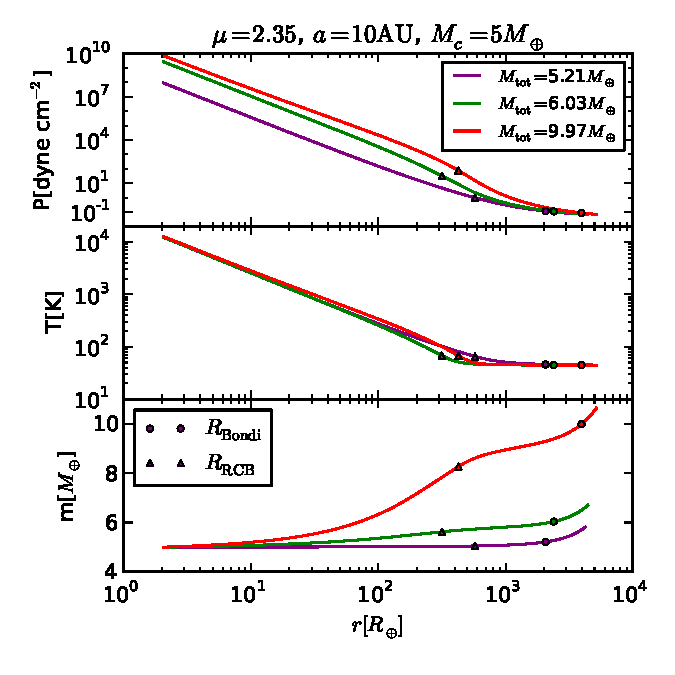
\includegraphics[width=0.5\textwidth]{../../figs/ModelAtmospheres/RadSelfGravPoly/PaperFigs/PTm_profiles_v2.pdf}
%%%\vspace{-0.5in}
%%\caption{Example pressure, temperature and mass profiles as a function of radius.}
%%\end{figure}
%
%The location of the Bondi radius moves further out as the mass of the atmosphere increases, as the Bondi radius scales with mass. The location of the radiative-convective boundary has a more interesting behavior. As stated in section \ref{intro}, the nebular gas initially settles into equilibrium around the protoplanetary core on a short timescale relative to the thermal timescale, and is isentropic throughout with an entropy equal to that of the disk. In the context of our model, this atmosphere represents the minimum atmosphere mass for which a hydrostatic solution exists. This atmosphere is purely convective. As gas accumulates and the atmosphere starts cooling, an outer radiative region forms. This layer is thin for low mass atmospheres, as can be seen in Fig. 1: for the $5.21 M_{\oplus}$ atmosphere, the ratio between the thickness of the radiative and convective regions is low. An increase in atmosphere mass causes the radiative zone to expand and the convective region to contract. As more and more gas is accumulated, the convective zone eventually starts expanding again; however, the ratio between the radii of the radiative and convective regions continually increases with atmosphere mass, i.e. the radiative regions of these types of atmospheres are getting deeper and deeper.  \textbf{[This needs to be rephrased, somewhat vague and repetitive.]}
%
%We further use the global cooling model developed in section \ref{cooling} to obtain an evolutionary series from static atmosphere profiles. Figure 2 shows the luminosity and cooling time evolution with atmosphere mass. Gas accretion is initially rapid, but slows down significantly after a relatively small mass increase. For comparison, we also plot the analytic results derived in section \ref{analytic}. We see that there is only a very brief agreement between the analytic and full numerical results. At early times, the radiative zone is too shallow and so the approximation that $P_{\rm RCB} \gg P_{\rm d}$ used in section \ref{analytic} breaks down. At late times, the self-gravity of the atmosphere becomes important. %We see that self-gravity starts to matter 
%
%%\begin{figure}[h]
%%\centering
%%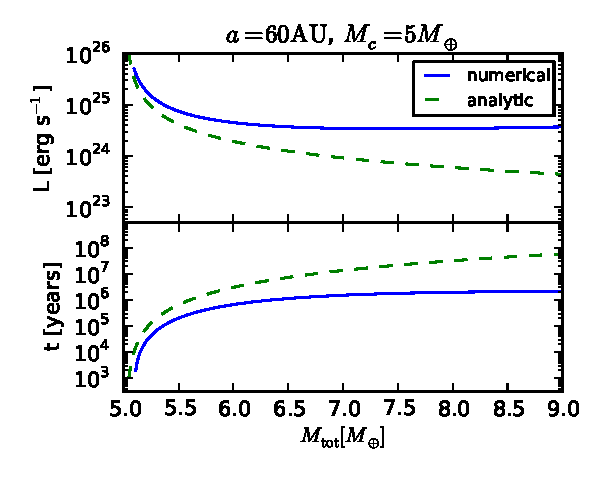
\includegraphics[width=0.5\textwidth]{../../figs/ModelAtmospheres/RadSelfGravPoly/PaperFigs/Lt_profiles_v2.pdf}
%%%\vspace{-0.5in}
%%\caption{Luminosity and time evolution with mass. The analytic result is plotted for comparison.}
%%\end{figure}
%
%%\subsection{The End of Quasi-Static Evolution}
%%\label{endoftime}
%%
%%
%%The right-hand side of equation (\ref{eq:dti}) decreases with increasing atmosphere mass, and eventually becomes negative when the mass of the envelope becomes comparable to the core mass $M_{\rm{atm}} \sim M_{\rm{c}}$. This implies a negative luminosity from the RCB. Physically, the luminosity $L$ represents the total heat flux through the surface defined by the RCB. The heat flux due to convective motions is always directed outwards, and hence it is positive. Moreover, the temperature gradient $dT/dr$ is negative, as the temperature decreases towards the outside. As a result (see equation (\ref{eq:structd})), the heat flux due to radiative diffusion is also positive. This implies that, in the absence of planetesimal accretion and internal heat sources, there is no physical mechanism that can justify a negative luminosity. The quasi-static, constant luminosity approximation breaks down at this point and a more detailed, time-dependent model is necessary.
%
%
%%As can be inferred from Figure 2, the time steps between subsequent evolutionary models become increasingly smaller as the atmosphere grows in mass. Around the time when the atmosphere mass is comparable to the core mass $M_{\mathrm{atm}} \sim M_{\mathrm{c}}$, we find that the time steps become negative.  

\section{Adiabatic Gradient for the Tabulated Equation of State}
\label{deladtable}

%\textbf{Explain the effects separately: dissociation vs. spin effects; show plots that explore these effects separately.}

%\subsection{Interpretation of Adiabatic Gradient Table}
%\label{deladinterp}

In this section we explain the differences in the behavior of thermodynamic variables between an ideal gas polytrope and a realistic equation of state by studying the dependence of the adiabatic gradient (defined in equation \ref{eq:delad}) on temperature and pressure. Figure \ref{fig:deladmap} shows a contour plot of the adiabatic gradient as a function of gas temperature and pressure, which was obtained by interpolating and extending the \citet{saumon95} equation of state tables as referenced in section \ref{sec2} and described in \App{EOStables}.

We distinguish three separate temperature regimes:


%In this section we aim to explain how the variable adiabatic index of the hydrogen-helium mixture described by a real equation of state affects the atmosphere evolution when compared to an ideal gas with constant $\delad$. A contour plot of the adiabatic gradient as extrapolated from the \citet{saumon95} EOS tables is shown in Figure \ref{fig:deladmap}. We distinguish three separate regimes:

\begin{enumerate}
\item Intermediate temperature regime (300 K $\lesssim T \lesssim 3000$), where the hydrogen-helium mixture behaves as an ideal gas characterized by a polytropic equation of state.
\item High temperature regime ($T \gtrsim$ 3000 K), where dissociation of molecular hydrogen occurs, followed by ionization of atomic hydrogen.
\item Low temperature regime ($T \lesssim 300$ K), where the temperature becomes low enough for rotational motion to reduce.
\end{enumerate}

We note that helium behaves like an ideal monatomic gas in our regime of interest ($\delad=2/5$). As such, its presence in the atmosphere only causes a small, constant upper shift in the adiabatic gradient of the mixture.

\begin{figure}[h]
\centering
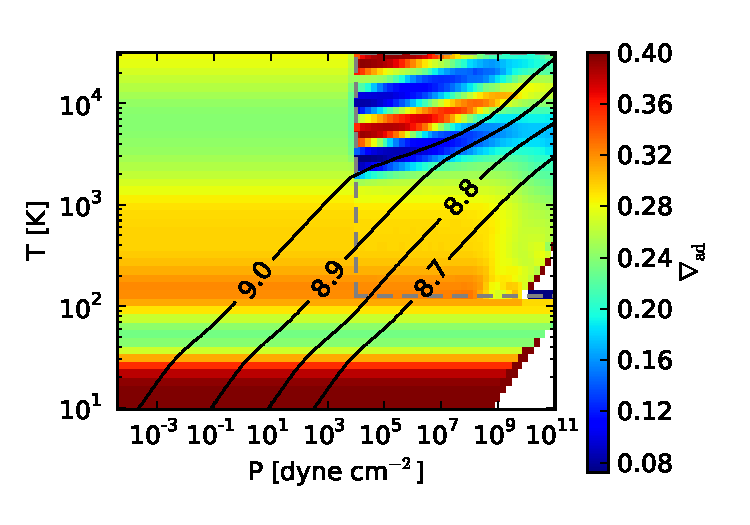
\includegraphics[width=0.5\textwidth]{../../figs/EOS/delad_S_mixt.pdf}
%%\vspace{-0.5in}
\caption{Contour plot of the adiabatic gradient $\delad$ for a hydrogen-helium mixture as a function of gas temperature and pressure. The upper right rectangle encloses the region described by the original \citet{saumon95} EOS tables, while the rest of the plot is our extension to lower temperatures and pressures. The black curves represent constant entropy adiabats, with the labels the natural logarithm of the absolute entropy per unit mass. At high temperatures, hydrogen dissociates and ionizes, while at low temperatures the rotational states of the hydrogen molecule are only partially excited and it therefore no longer behaves like an ideal diatomic gas. The discontinuity between the original EOS tables and our extension is due to the fact that we did not take into account dissociation and ionization. However, in our regime of interest (encompassed by the constant entropy curves), the extension matches smoothly with the original tables.}
\label{fig:deladmap}
\end{figure}

In what follows we explain the behavior of the adiabatic gradient in the three temperature regimes separately.

\vspace{0.2in}

\textbf{1. Intermediate T: Ideal Gas}

For temperatures less than $\sim 2000$ K but larger than $\sim 300$ K, the hydrogen molecule is not energetic enough to dissociate and hydrogen behaves as an ideal diatomic gas. We see this in Fig. \ref{fig:deladmap} for 300 K $\lesssim T \lesssim 3000$ K, where the adiabatic gradient is approximately constant. The helium component of the gas causes a slight increase in the adiabatic index: $\delad \approx 0.3$ in this temperature range rather than 2/7 as is the case for a diatomic gas.

\vspace{0.2in}

\textbf{2. High T: Dissociation and Ionization of Hydrogen.}

At low temperatures, hydrogen exists in molecular form, which has a stable configuration. As the temperature becomes higher than $T \sim 2000-3000$ K, the internal energy becomes large enough to break the covalent bond between the atoms, and hydrogen starts dissociating. At temperatures of the order of $10^4$ K, the internal energy becomes large enough to remove electrons from the atoms, and hydrogen ionizes. In stellar and giant planet interiors there is little overlap between the two processes: hydrogen is almost entirely dissociated into atoms by the time ionization becomes important. 

For a mixture of molecular and atomic hydrogen, we expect the adiabatic gradient to have an intermediate value between monatomic and diatomic gas, while for a mixture of protons and electrons the adiabatic index is just $2/5$ as for a monatomic ideal gas. However, we notice in Fig. \ref{fig:deladmap} that the adiabatic gradient decreases significantly in the regions where hydrogen is either partially dissociated or partially ionized. We further explain this behavior.

We first discuss ionization. For a mixture of ideal gases, the total internal energy is given by the sum of the internal energies of the individual gases. When a gas is ionized, however, the energy used to ionize the atoms has to also be taken into account. This energy depends on the ionization fraction and can be determined from the Saha equation (see e.g., \citealt{kippenhahn90}). The ionization fraction only depends on gas temperature and density (see \App{deladioniz}), and hence only the equation of state. An expression of the adiabatic gradient as a function of the ionization fraction can be derived. We present this expression in \App{deladioniz}. The adiabatic gradient is $\delad=2/5$ when there is no ionization (i.e., only atomic hydrogen) or when the plasma is fully ionized, but decreases significantly during partial ionization, reaching a minimum when half of the gas is ionized. 

This is consistent with the behavior we see in Figure \ref{fig:deladmap}. At constant entropy, we expect an increase in pressure to increase the internal energy of the system, thus causing the temperature to also rise significantly. In the case of partial ionization, however, part of the internal energy is used to remove the electrons from atoms, and therefore there is less energy available to increase the temperature of the system. This behavior of the constant entropy curves is seen in Figure \ref{fig:deladmap}. 


The dissociation of molecular hydrogen is dictated by an equation similar to the Saha equation, with the ionization energy replaced by dissociation energy (equal to 4.27 eV for molecular hydrogen, \citealt{mandl89}). The adiabatic gradient therefore has an analogous behavior, consistent with Fig. \ref{fig:deladmap}.


%We now investigate the effect of the low adiabatic index caused by hydrogen dissociation on the luminosity and cooling time evolution of the atmosphere. The left panel of Figure (x) shows the 

%The resulting luminosity and time evolution are shown in Figure \ref{fig:Ltplotall}. We use again instantaneous atmosphere profiles to explain the differences. Figure \ref{fig:ETrprofall} shows the instantaneous temperature and energy profiles, as well as the location of the Bondi radius for a total fixed mass $M_{\rm{tot}}=11.8 M_{\oplus}$. We see that the spin effect at the outer boundary dictates the location of the radiative zone, and therefore the luminosity behavior, while dissociation deep in the atmosphere dictates the energy behavior. As compared to the polytrope, the real EOS therefore generates a deeper radiative zone with a lower luminosity, due to the lower adiabatic index in the outer regions, as well as an atmosphere with the bulk of its energy concentrated at the bottom, due to the low $\delad$ caused by dissociation. As shown above for the ideal gas polytropes, and remembering that $\Delta t \sim -\Delta E/L$, we see that both effects result in a longer time for the atmosphere to evolve.  


\vspace{0.2in}

\textbf{3. Low T: Hydrogen Rotation and Spin Isomers}

As a diatomic molecule, hydrogen has five degrees of freedom, three associated with translational motion and two associated with rotation. At room temperature, the rotational states are fully excited and the full rotational effects are seen. The excitation temperature for rotation is $\Theta_r \approx 85$ K for the hydrogen molecule (e.g., \citealt{kittel}); as the gas temperature becomes comparable to $\Theta_r$, fewer rotational states are excited and rotation entirely ceases as $T \rightarrow 0$. %Here we explore the quantum mechanical effects associated with rotation. %We present expressions for the partition function associated with rotation and derive relevant thermodynamic variables in \App{EOStables}. For $T \ll \Theta_r$, the partition function is just equal to one, and no rotational states are excited for very low temperatures and hydrogen behaves like a monatomic gas. On the other hand, if $T \gg \Theta_r$, the molecule is energetic enough for all the rotational states to be fully excited. 

In this section we discuss the quantum effects of the hydrogen isomeric forms and the way they affect the rotational energy and heat capacity of the hydrogen molecule at low temperatures, and hence the adiabatic gradient. 

 Molecular hydrogen occurs in two isomeric forms: orthohydrogen, with parallel proton spins, and parahydrogen, with antiparallel proton spins. The Pauli exclusion principle requires the total wavefunction of two fermions, such as protons, to be antisymmetric. As such, a symmetric spin wavefunction requires an antisymmetric rotational wavefunction, and vice-versa (\citealt{farkas35}). Parahydrogen has an antisymmetric spin wavefunction, which means that it can only occupy symmetric rotational states and hence the angular quantum number $j$ has to be even. By analogy, orthohydrogen must have an antisymmetric rotational wavefunction and can only occupy states with odd $j$. The partition functions for ortho- and parahydrogen are described in \App{EOStables}.
 At equilibrium, the relative abundance of the ortho and para states is given by the ratio of their partition functions. For very low temperatures there is only parahydrogen, as molecules are in the ground state with $j=0$, which corresponds to the para state. As the temperature is increased, parahydrogen starts converting into orthohydrogen, resulting in an ortho-para equilibrium ratio of 3:1 at room temperature.

%\begin{figure}[h]
%\centering
%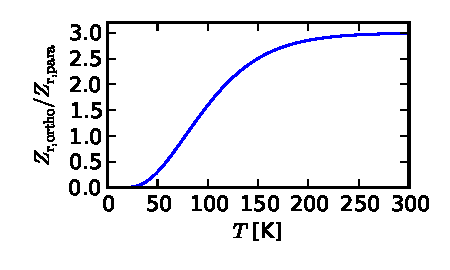
\includegraphics[width=0.5\textwidth]{../../figs/ModelAtmospheres/RadSelfGravRealEOS/EOSeffects/ortho_para_ratio.pdf}
%%%\vspace{-0.5in}
%\caption{Relative abundance of ortho- and parahydrogen as a function of temperature.}
%\label{fig:Zrel}
%\end{figure}

The internal energy and specific heat per unit mass associated with rotation for the individual isomers and for the equilibrium mixture can be derived from equations (\ref{eq:Zpara}), (\ref{eq:Zortho}), (\ref{eq:Zrspin}), (\ref{eq:u}) and (\ref{eq:cv}) and plotted in Figure \ref{fig:ucvr}. The para state has no rotational energy for low temperatures, since all the molecules occupy the rotational level with $j=0$. Orthohydrogen, on the other hand, is in the $j=1$ state, and so has an energy given by the energy of its first rotational level. Since all the hydrogen mixtures behave like monatomic gases at low temperatures, their rotational heat capacity is zero in this region. This is consistent with $\delad=2/5$ at low temperatures as seen in Fig. \ref{fig:deladmap}. There are two significant maxima in the heat capacities of parahydrogen and of the mixture. At very low temperatures, the heat capacity of parahydrogen is zero because only the lowest accessible energy level $j=0$ is occupied and a temperature increase does not provide enough energy to populate the next higher level. When the temperature becomes sufficiently high to populate the second lowest level $j=2$, the heat capacity rapidly increases, passes through a maximum and starts to decrease when the second lowest level becomes saturated. The maxima in the ortho-para mixture appears around the time when parahydrogen starts converting into orthohydrogen. The heat capacity of the equilibrium mixture is not a weighted average of the heat capacities of the individual components because it takes into account both the rotational energy uptake of para- and ortho-hydrogen, and also the shift in their equilibrium concentrations with temperature. At $T=0$, only para-hydrogen is present in the equilibrium mixture; as the temperature is increased, the energetically higher-lying ($j=1$) ortho-hydrogen is formed, and the concomitant energy increase is seen as a peak in the heat capacity. As the adiabatic gradient is inversely proportional to the heat capacity, it means that  the former has to first decrease from 2/5 as the temperature increases, reach a minimum around 50 K ($\delad \approx 0.25$ from Fig. \ref{fig:deladmap}), then gradually increase to 2/7 as for a diatomic gas. This behavior is illustrated in Fig. \ref{fig:deladmap}.  


\begin{figure}[h]
\centering
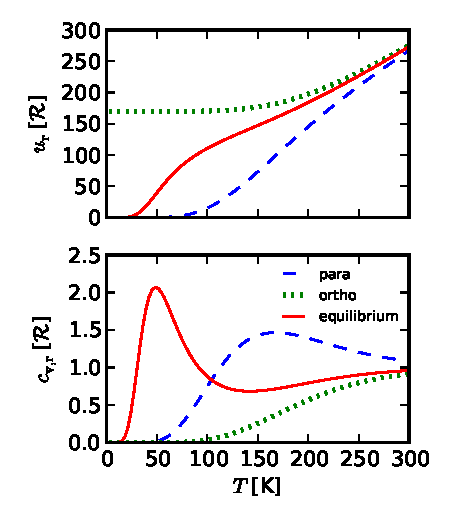
\includegraphics[width=0.5\textwidth]{../../figs/ModelAtmospheres/RadSelfGravRealEOS/EOSeffects/ortho_para_energy.pdf}
%%\vspace{-0.5in}
\caption{Internal energy and heat capacity per unit mass for the hydrogen spins isomers and the equilibrium mixture as a function of temperature.}
\label{fig:ucvr}
\end{figure}



%\vspace{0.1in}

\section{Equation of State Effects on Atmosphere Evolution}
\label{EOSeffects}

Variations in the adiabatic gradient have two competing effects on the atmosphere evolution: they affect the luminosity of the envelope and the amount of energy needed to accrete more mass, i.e. $dE/dM$. Together, they result in changes in the growth time of the atmosphere, and therefore in the crossover time and critical core mass. In this section we discuss how the variable adiabatic gradient discussed in section \ref{deladtable} affects the atmosphere evolution when compared to an ideal gas of constant $\delad$. We explore the effect of partial dissociation and hydrogen spin isomers (see section \ref{deladtable}) on the atmosphere luminosity and cooling time evolution. As the adiabatic gradient is variable throughout the atmosphere profiles described in section (\textbf{some previous section}), we first investigate the differences in atmosphere profiles and evolution for ideal gas polytropes with different adiabatic gradients in section \ref{deladpoly}. We then show how the variable adiabatic gradient affects the time evolution of the atmosphere in section \ref{deladeffect}.

\subsection{Ideal Gas Polytropes with Different Adiabatic Gradient}
\label{deladpoly}

In this section we investigate the differences in luminosity and $dE/dM$, and the resulting time evolution, between ideal gas polytropes with different adiabatic gradients: $\delad=2/7$ (diatomic gas) and $\delad=2/5$ (monatomic gas). We assume both gases have the same mean molecular weight. %We use these results to explain the separate effects of dissociation and spin on the time evolution of the atmosphere.

We generate atmosphere profiles for the two different adiabatic indices at $a=10$ AU and for a core mass $M_{\rm c}=10 M_{\oplus}$, and estimate the luminosity and cooling time evolution as described in section \ref{sec2}. The results are shown in Figure \ref{fig:Ltplotpoly}. We find that the polytrope with the lower adiabatic gradient has both a higher luminosity and a longer cooling time. We use instantaneous atmosphere profiles to explain these effects. 

We first discuss the effect of the variable adiabatic gradient on luminosity. Figure \ref{fig:ETrplotpoly}, top panel, shows the temperature profile as well as the location of the radiative-convective boundary for the two polytropes at a fixed total mass $M_{\rm{tot}}=11.8 M_{\oplus}$. The polytrope with a larger adiabatic gradient has a more shallow convective zone, and hence a deeper radiative region, since a larger temperature gradient delays the onset of convection. As the luminosity in the radiative region is inversely proportional to the depth of the radiative zone (see equation (\ref{eq:structd})), a deeper radiative region results in a lower luminosity, which explains the results in the top panel of Figure \ref{fig:Ltplotpoly}. 

\begin{figure}[h]
\centering
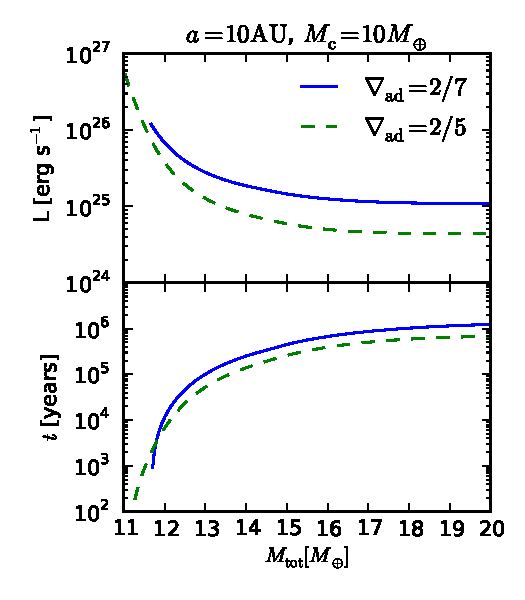
\includegraphics[width=0.5\textwidth]{../../figs/ModelAtmospheres/RadSelfGravRealEOS/EOSeffects/Ltplot_poly.pdf}
%%\vspace{-0.5in}
\caption{Luminosity and time evolution as a function of total mass (core + atmosphere) for polytropes with different adiabatic indices, for a planet forming at 10 AU and with a fixed core mass $M_{\rm c}=10 M_{\oplus}$. A larger adiabatic index results in both a lower luminosity and a shorter cooling time.}
\label{fig:Ltplotpoly}
\end{figure}

\begin{figure}[h]
\centering
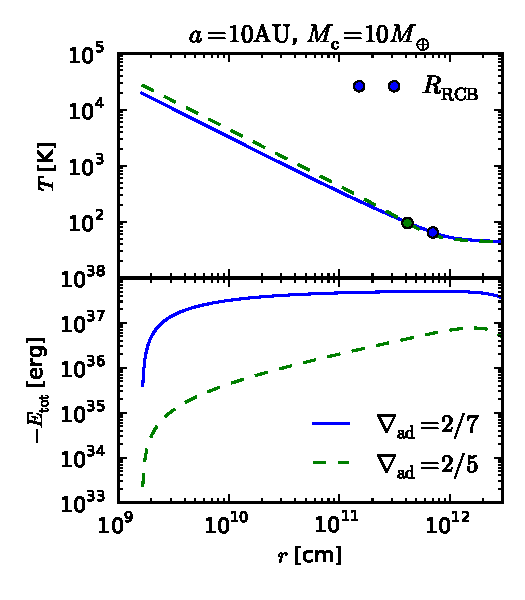
\includegraphics[width=0.5\textwidth]{../../figs/ModelAtmospheres/RadSelfGravRealEOS/EOSeffects/TErplot_poly.pdf}
%%\vspace{-0.5in}
\caption{Instantaneous temperature and total energy profiles as a function of radius for polytropes with different adiabatic indices, for a planet forming at 10 AU and with a fixed core mass $M_{\rm c}=10 M_{\oplus}$. The total mass (core + atmosphere) is $11.8 M_{\oplus}$. The location of the radiative-convective boundary is marked. A lower adiabatic gradient results in a more shallow radiative region (upper panel), and in the total energy being concentrated at the bottom of the atmosphere (lower panel).}
\label{fig:ETrplotpoly}
\end{figure}

We study the energy behavior for the two polytropes in order to explain the $dE/dM$ effect. We have shown in Piso \& Youdin (in prep.) that polytropes with $\delad=2/7$ have most of the energy concentrated at the bottom of the atmosphere, while polytropes with $\delad=2/5$ have the bulk of the energy towards the outer boundary. The bottom panel of Figure \ref{fig:ETrplotpoly} shows an instantaneous energy profile for the same total mass $M_{\rm{tot}} = 11.8 M_{\oplus}$, confirming this behavior. It takes more energy to bring in gas deep in the atmosphere for an envelope that has the bulk of its energy concentrated towards the bottom,  resulting in a larger $dE/dM$. The energy effect prevails over the luminosity effect, resulting in a longer cooling time for the envelope, as shown in the bottom panel of Figure \ref{fig:Ltplotpoly}.


%From the adiabatic gradient table shown in Figure \ref{fig:deladmap} we find that $\delad$ has the flattest behavior around $T=500$ K. In this region, the gas behaves like an ideal gas with constant polytropic index $\delad \approx 0.3$, with the shift from diatomic gas caused by the helium in the mixture. We generate three sets of atmosphere profiles. The first one corresponds to an ideal gas of constant adiabatic index $\delad=0.3$. The second one is described by the real EOS for temperatures larger than 500 K and by an ideal gas with $\delad=0.3$ for $T<500$ K. Finally, the third profile consists of an ideal gas polytrope with $\delad=0.3$ for $T>500$ K and a real gas in the low temperature regime. We compare the first two profiles to show the dissociation effects, and the first and third profile to show the effects of ortho- and parahydrogen. The resulting time evolution is shown in Figure \ref{fig:Ltplotall}. We see that both dissociation and spin isomers have a comparable effect on the atmosphere growth, and result in slower cooling, and therefore a longer crossover time, when compared to the polytropic ideal gas equation of state. In what follows we explore the two effects separately.



%\subsection{Effect of Adiabatic Gradient on Atmosphere Cooling Time}
%\label{deladeffect}

%In this section we discuss the effect of the variable adiabatic index described in subsection \ref{deladinterp} on the atmosphere cooling time. 

%We now explore the separate effects of hydrogen dissociation at high temperatures and spin isomers at low temperatures. From the adiabatic gradient table shown in Figure \ref{fig:deladmap} we find that $\delad$ has the flattest behavior around $T=500$ K. In this region, the gas behaves like an ideal gas with constant polytropic index $\delad \approx 0.3$, with the shift from diatomic gas caused by the helium in the mixture. We generate three sets of atmosphere profiles. The first one corresponds to an ideal gas of constant adiabatic index $\delad=0.3$. The second one is described by the real EOS for temperatures larger than 500 K and by an ideal gas with $\delad=0.3$ for $T<500$ K. Finally, the third profile consists of an ideal gas polytrope with $\delad=0.3$ for $T>500$ K and a real gas in the low temperature regime. We compare the first two profiles to show the dissociation effects, and the first and third profile to show the effects of ortho- and parahydrogen. 

%We now explore the effects of 

\subsection{Dissociation and Spin Isomers Effects}
\label{deladeffect}

We now discuss the differences in luminosity and $dE/dM$ between an ideal gas with constant adiabatic gradient and atmospheres with variations in $\delad$ as prescribed by the equation of state discussed in section \ref{EOSeffects}. In what follows we describe our choices of equation of state combinations. From the adiabatic gradient table shown in Figure \ref{fig:deladmap} we find that $\delad$ has the flattest behavior around $T=500$ K. In this region, the gas behaves like an ideal gas with constant polytropic index $\delad \approx 0.3$, with the shift from diatomic gas caused by the helium in the mixture. We generate three sets of atmosphere profiles. The first one corresponds to an ideal gas of constant adiabatic index $\delad=0.3$. The second one is described by the real EOS for temperatures larger than 500 K and by an ideal gas with $\delad=0.3$ for $T<500$ K. Finally, the third profile consists of an ideal gas polytrope with $\delad=0.3$ for $T>500$ K and a real gas in the low temperature regime. We compare the first two profiles to show the dissociation effects, and the first and third profile to show the effects of ortho- and parahydrogen. The resulting time evolution is shown in Figure \ref{fig:tplotall}. We see that both dissociation and spin isomers have a comparable effect on the atmosphere growth, and result in slower cooling, and therefore a longer crossover time, when compared to the polytropic ideal gas equation of state. The cooling time is dependent on both the total energy released due to the contraction of the envelope and the luminosity of the atmosphere. In what follows we explore the relative influence of these two factors separately.

\begin{figure}[h]
\centering
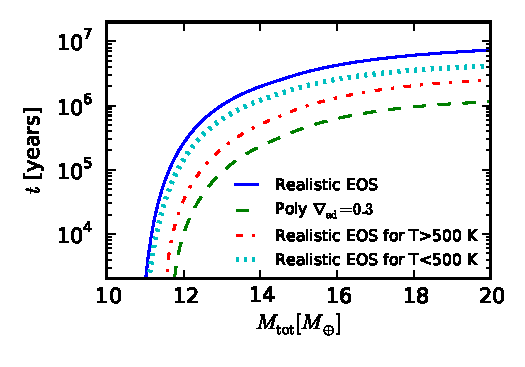
\includegraphics[width=0.5\textwidth]{../../figs/ModelAtmospheres/RadSelfGravRealEOS/EOSeffects/tplot.pdf}
%%\vspace{-0.5in}
\caption{Cooling time evolution as a function of total mass (core + atmosphere) for a variety of EOS combinations, for a planet forming at 10 AU and with a fixed core mass $M_{\rm c}=10 M_{\oplus}$. The cooling time is larger both due to hydrogen dissociation and spin effects when compared to an ideal gas polytrope.}
\label{fig:tplotall}
\end{figure}

%We now investigate the effect of the low adiabatic index caused by hydrogen dissociation, on the one hand, and spin isomers on the other hand, on the luminosity and cooling time evolution of the atmosphere, in light of the discussion in section \ref{deladpoly}. The left panel of Figure (x) shows the luminosity evolution with mass for the four combinations of equations of state described in section  

The right panel of Figure \ref{fig:TLrplot} shows the luminosity evolution with mass for the three combinations of equations of state described above, as well as for the complete real gas EOS. We use again instantaneous atmosphere profiles to explain the differences. The left panel of Figure \ref{fig:TLrplot} shows the instantaneous temperature profile and the location of the radiative-convective boundary for a total fixed mass $M_{\rm{tot}}=11.8 M_{\oplus}$. The real equation of state for low temperatures is characterized by a lower adiabatic index in the outer regions, due to the spin effects, and is therefore dominant in the radiative zone. As a result, it generates a deeper radiative zone with a lower luminosity, which explains the results in the left panel of Figure \ref{fig:TLrplot}. Moreover, since the cooling time is inversely proportional to the luminosity, the spin effect will result in a longer cooling (and crossover) time.

The energy behavior is shown in Figure \ref{fig:Erplot}. The real EOS for high temperatures has a low adiabatic index deep in the atmosphere, due to hydrogen dissociation, and thus the bulk of its energy concentrated at the bottom of the atmosphere, for the reasons described in section \ref{deladpoly}. It takes more energy to add mass more mass deep in the atmosphere, and $dE/dM$ is larger as a result. 
%

We have seen that the spin effect at the outer boundary dictates the location of the radiative zone, and therefore the luminosity behavior, while dissociation deep in the atmosphere dictates the energy behavior. Overall, both effects result in a longer time for the atmosphere to evolve. 

%As compared to the polytrope, the real EOS therefore generates a deeper radiative zone with a lower luminosity, due to the lower adiabatic index in the outer regions, as well as an atmosphere with the bulk of its energy concentrated at the bottom, due to the low $\delad$ caused by dissociation. As shown above for the ideal gas polytropes, and remembering that $\Delta t \sim -\Delta E/L$, we see that both effects result in a longer time for the atmosphere to evolve.  

\begin{figure*}[tb]
\centering
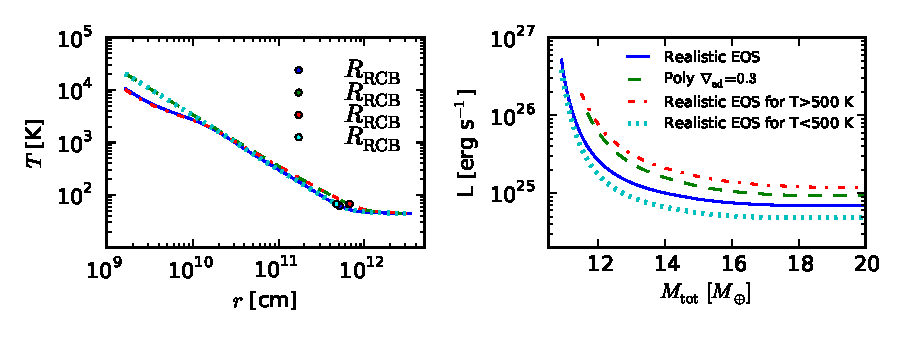
\includegraphics[width=\textwidth]{../../figs/ModelAtmospheres/RadSelfGravRealEOS/EOSeffects/TLr_plot.pdf}
%%\vspace{-0.5in}
\caption{Left panel: Instantaneous emperature profile as a function of radius for a variety of EOS combinations, for a planet forming at 10 AU and with a fixed core mass $M_{\rm c}=10 M_{\oplus}$. The total mass (core + atmosphere) is $11.8 M_{\oplus}$. The location of the radiative-convective boundary is marked. The effect of hydrogen spin isomers in the outer region of the atmosphere sets the location of the radiative-convective boundary.  Right panel: Luminosity evolution as a function of total mass (core + atmosphere) for a variety of EOS combinations, for a planet forming at 10 AU and with a fixed core mass $M_{\rm c}=5 M_{\oplus}$. Dissociation deep in the atmosphere increases the luminosity when compared to an ideal gas polytrope, while the existence of the hydrogen spin isomers in the outer part of the atmosphere results in a lower luminosity. The two effects combined yield a lower luminosity for the realistic equation of state when compared to the polytrope. }
\label{fig:TLrplot}
\end{figure*}

\begin{figure}[h]
\centering
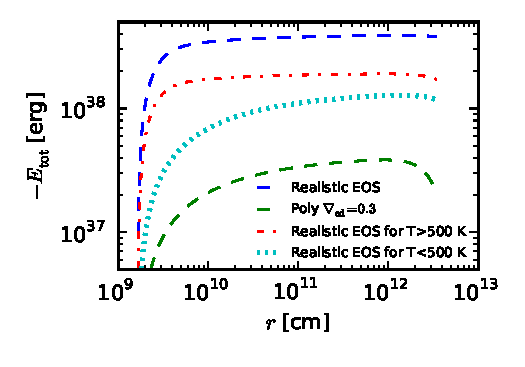
\includegraphics[width=0.5\textwidth]{../../figs/ModelAtmospheres/RadSelfGravRealEOS/EOSeffects/Er_plot.pdf}
%%\vspace{-0.5in}
\caption{Instantaneous energy profiles as a function on radius for a variety of EOS combinations, for a planet forming at 10 AU and with a fixed core mass $M_{\rm c}=10 M_{\oplus}$. The total mass (core + atmosphere) is $11.8 M_{\oplus}$. Hydrogen dissociation deep in the atmospheres causes the bulk of the energy to be concentrated at the bottom of the atmosphere.}
\label{fig:Erplot}
\end{figure}





%\subsection{Outer Boundary Effects}

%\textbf{Reemphasize the fact that the atmosphere structure is determined by your outer boundary conditions: T_{out}, P_{out}, R_{out} $\rightarrow$ explore the separate effects of pressure, temperature and a (since the Hill radius is determined by a); show how temperature is the strongest effect. }

\section{Critical Core Mass}
\label{critical}

%\textbf{Define what it is (refer again to paper I also); show the Mcrit vs a for fixed disk life plot, for both real EOS, gamma 7/5 and gamma 5/3; justify the differences in terms of the EOS effects from 4.2; show that using a real EOS makes a significant difference to the results; however, the core masses we get are still doable. Again, a lot of text below will be used but needs reorganizing/rephrasing.}

%\textbf{Define what it is (also refer to paper I) and emphasize how it's different from $M_{crit}$ in standard calculations. Define the crossover mass and crossover time.}


In this section we put together the results obtained in section \ref{EOSeffects} and determine the minimum core mass to initiate runaway gas accretion during the lifetime of the protoplanetary disk assuming that the nebular gas is described by a realistic equation of state as prescribed by the \citet{saumon95} EOS tables (see section \ref{EOSeffects}). As in Piso \& Youdin (in prep.), we define this minimum core mass as the \textit{critical core mass}. Moreover, we define the time elapsed until runaway gas accretion is initiated when $M_{\rm{atm}} \sim M\co$ as the \textit{crossover time}. In this section we first explore the dependence of the crossover time on the core mass for a fixed semi-major axis. We then determine the critical core mass to form a giant planet before the dissipation of the gas in the protoplanetary disk, assuming that the nebular gas is described by a realistic hydrogen-helium mixture, and we compare this with the results from Piso \& Youdin (in prep.) for an ideal diatomic gas. 

%\subsection{Crossover Time as a Function of Core Mass}
%\label{tvsM}

%\textbf{t vs. M at fixed distance, similar to the plot from paper I. Compare scalings.}

Figure \ref{fig:tvsMplot} displays the time evolution and the crossover time for core masses between 7 and 16 $M_{\oplus}$ at $a=10$ AU in our fiducial disk. The crossover time is shorter for lower mass cores, consistent with the results of Piso \& Youdin (in prep.). 

\begin{figure}[h!]
\centering
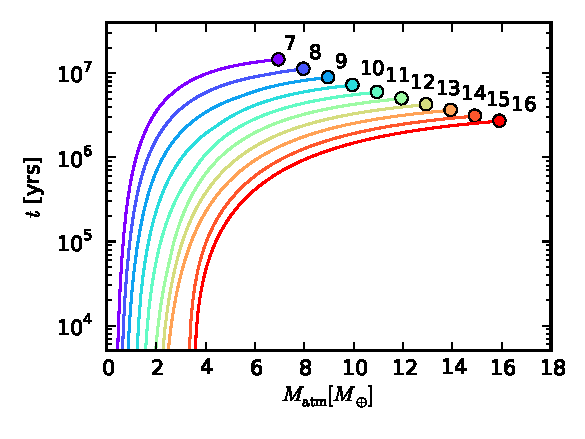
\includegraphics[width=0.5\textwidth]{../../figs/ModelAtmospheres/RadSelfGravRealEOS/t_vs_M_10au.pdf}
%%\vspace{-0.5in}
\caption{Time to grow an atmosphere of mass $M_{\rm{atm}}$ for cores with fixed masses between $7 M_{\oplus}$ and $16 M_{\oplus}$ at $a=10$ AU in our fiducial disk. The circles mark the crossover time where $M_{\rm{atm}} \sim M_{\rm c}$. The numbers are labeling the core mass in Earth masses. A larger core mass results in a shorter crossover time.}
\label{fig:tvsMplot}
\end{figure}

%\subsection{Critical Core Mass}
%\label{Mcrit}

%\textbf{Mcrit vs. a plot, realistic EOS and polytrope. Discuss the larger critical core mass for the real EOS in light of the effects from section 4.}

Figure \ref{fig:Mvsaplot} shows the critical core mass for a massive atmosphere to form during a typical lifetime of a protoplanetary disk $t=3$ Myrs, for a gas described by a realistic equation of state. For comparison, we also plot the results of Piso \& Youdin (in prep.) for an ideal diatomic gas. The use of a realistic equation of state increases the critical core mass by more than a factor of 2. As such, non-ideal effects substantially affect the core mass needed to form a giant planet  before the dissipation of the protoplanetary disk.   

\begin{figure}[h!]
\centering
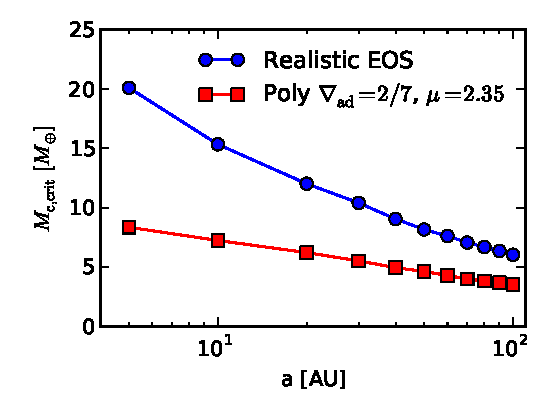
\includegraphics[width=0.5\textwidth]{../../figs/ModelAtmospheres/RadSelfGravRealEOS/Mc_vs_a_poly_real_paper.pdf}
%%\vspace{-0.5in}
\caption{The minimum core mass for an atmosphere to initiate runaway gas accretion within the lifetime of a typical protoplanetary disk $t \sim 3$ Myrs as a function of semi-major axis, for a realistic hydrogen-helium mixture. The results of Piso \& Youdin (in prep.) for an ideal diatomic gas are plotted for comparison. The realistic equation of state yields core masses larger by more than a factor of 2 when compared to the polytrope.}
\label{fig:Mvsaplot}
\end{figure}


\section{Model Relevance in Planet Formation Theory}
\label{acc}

In this study we have considered atmospheres for which planetesimal accretion is negligible and Kelvin-Helmholtz contraction dominates the luminosity evolution of the atmosphere. This is different from standard calculations, in which the atmosphere is heated by planetesimal accretion. In this section we compare our results for the critical core mass to analogous results from the standard calculations. We discuss the core accretion rates that are necessary for our regime to be valid in section \ref{raf1}. We then compare our results with planetesimal accretion results under similar assumptions in section \ref{raf2}.

 %In this section we investigate the core accretion rates that are necessary for our regime to be valid. We also discuss the conditions under which runaway gas accretion can be initiated due to the Kelvin-Helmholtz contraction of the atmosphere before it becomes critical due to planetesimal accretion.

\subsection{Planetesimal Accretion Rates}
\label{raf1}

We estimate the planetesimal accretion rate consistent with our assumptions that $L_{\mathrm{acc}} \ll L_{\rm{KH}}$. Here $L_{\rm{acc}}$ is the accretion luminosity given by

\begin{equation}
\label{eq:Lacc}
L_{acc}=G \frac{M_{\rm{c}} \dot{M_{\rm{c}}}}{R_{\rm{c}}},
\end{equation}

\noindent where $\dot{M_{\rm{c}}}$ is the planetesimal accretion rate, and $L_{\rm{KH}}$ is the luminosity of the atmosphere due to gas contraction obtained from our static model described in section \ref{sec2}. At the limit, $L_{\rm{acc}}=L_{\rm{KH}}$. For a given atmosphere model we can therefore estimate the maximum planetesimal accretion rate during the gas contraction phase in order for the atmosphere to be dominated by gas contraction. We choose as a fiducial case an atmosphere forming at 40 AU and with a core mass of $10 M_{\oplus}$, described by a realistic equation of state. For this choice of parameters, the atmosphere crossover time is $t \sim$ 2.7 Myrs, which is within the typical life time of a protoplanetary disk. The results are presented in Figure \ref{fig:accrates}. 

 \begin{figure}[h]
\centering
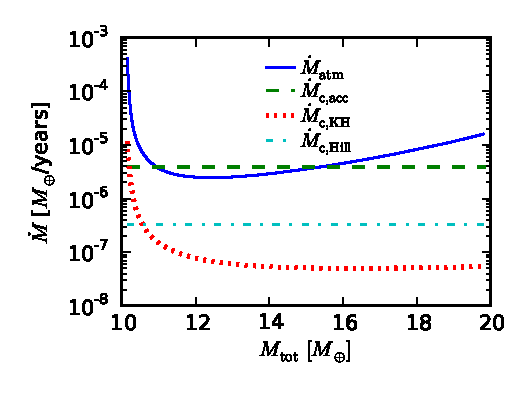
\includegraphics[width=0.5\textwidth]{../../figs/ModelAtmospheres/RadSelfGravPoly/acc_rates_paper.pdf}
%\vspace{-0.5in}
\caption{Various relevant accretion rates. $\dot{M}_{\rm{atm}}$ is the growth rate of the atmosphere as estimated by our model, and $\dot{M}_{\rm{c,KH}}$ is the maximum planetesimal accretion rate during the gas contraction phase in order for our regime to be valid. For comparison, we plot the core accretion rate $\dot{M}_{\rm{c,acc}}$ necessary to grow the core on the same time scale as the atmosphere $\tau \sim 2.7$ Myrs, and a typical planetesimal accretion rate where the random velocity of the planetesimals is given by the Hill velocity due to the core.}
\label{fig:accrates}
\end{figure}

We label the resulting minimum core accretion rate as $\dot{M}_{\rm{c,KH}}$. The atmosphere growth rate $\dot{M}_{\rm{atm}}$ is also plotted for comparison. We therefore see that the core accretion rate has to be $\sim2-3$ orders of magnitude lower than the atmosphere accretion rate for our assumptions to be valid.  If the core had accreted planetesimals at this constant rate since it started forming, then the formation of a core massive enough to attract an atmosphere would not have been possible within typical disk life timescales, which indicates a slowing down of the planetesimal accretion regime. Possible explanations for that include the core having formed in the inner part of the disk and later migrated outwards, or the core having been depleted of planetesimals due to a giant neighbor. We also estimate the core accretion rate 

\begin{equation}
\label{eq:Mcdot}
\dot{M}_{\rm{c,acc}}(M_{\rm{c}}) \equiv \frac{M_{\rm{c}}}{\tau}
\end{equation}

\noindent needed for the core to form on the same timescale as our model atmosphere, $\tau=2.7$ Myrs, as well as a typical planetesimal accretion rate, for which the random velocities of the planetesimals are of the order of the Hill velocity around the protoplanetary core \citep{goldreich04}. We denote this latter rate as $\dot{M}_{\rm{c,typical}}$. This is the accretion rate at the boundary between the dispersion dominated and shear dominated regimes. It is easy to see that  $\dot{M}_{\rm{c,typical}}$ is more than one order of magnitude lower than the gas accretion rate of our model atmosphere $\dot{M}_{\rm{atm}}$, and lower than the core accretion rate $\dot{M}_{\rm{c,acc}}$ needed to grow the core and the atmosphere at the same time within the disk life time. As such, the formation of a giant planet by growing the core first, then letting the atmosphere cool is faster than growing the core and the atmosphere at the same time at a steady planetesimal accretion rate.

\subsection{Comparison with Standard Results}
\label{raf2}

Next, we are interested in whether hydrodynamic gas accumulation due to planetesimal accretion can already commence before the atmosphere becomes unstable due to Kelvin-Helmholtz contraction, as our regime is no longer the relevant one under such conditions. A core that forms on the same timescale as our model atmosphere accretes planetesimals at a rate given by equation (\ref{eq:Mcdot}). This accretion rate is dependent on the core mass, which is steadily increasing. We therefore compare the critical core mass due to planetesimal accretion at this rate $M_{\rm{crit,acc}}$ to the critical core mass as defined in our estimates $M_{\rm{c,crit}}$ (see section \ref{critical}). If $M_{\rm{crit,acc}}<M{\rm_{c, crit}}$, then the atmosphere has already initiated unstable gas accretion by the time Kelvin-Helmholtz contraction starts dominating. 

%Specifically, we compare the critical core mass due to planetesimal accretion at the rate 

%we compare the critical core mass $M_{\rm{c,acc}}$ due to planetesimal accretion, for an accretion rate that satisfies $L_{\rm{acc}}<L_{\rm{KH}}$ to the actual core mass $M_{\rm{c}}$ assumed fixed in our model. If $M_{\rm{c,acc}}<M{\rm{c}}$, then the atmosphere has already initiated unstable gas accretion by the time Kelvin-Helmholtz contraction starts dominating. 

In order to estimate the critical core mass due to planetesimal accretion $M_{\rm{crit,acc}}$, we use the results of \citet{rafikov06} for low luminosity atmospheres forming in the outer disk ($>2-5$ AU), consistent with our region of interest. \citet{rafikov06} assumes an ideal gas polytropic equation of state and a lower opacity than the standard ISM opacity that we use in our calculations (see equation \ref{eq:opacitylaw}), due to grain growth. In Piso \& Youdin (in prep.) we showed that a reduction in opacity results in a shorter crossover time and therefore a lower critical core mass. In this section, we calculate the critical core mass for an ideal gas polytrope with the standard ISM opacity reduced by a factor of 100, which is comparable to the opacity law used by \citet{rafikov06}. 

By relating his expression for the critical core mass to a given core mass dependent planetesimal accretion rate $\dot{M}(M_{\rm{c}})$, we find the following expression for the critical core mass when accretion luminosity dominates the evolution of the atmosphere:

\begin{equation}
\label{eq:critraf}
M_{\rm{crit, acc}} \sim \Big[\frac{\dot{M}(M_{\rm{c}})}{64 \pi^2 C} \frac{\kappa_0}{\sigma G^3} \frac{1}{R\co M\co^{1/3}} \Big(\frac{k}{\mu}\Big)^4\Big]^{3/5},
\end{equation}

\noindent with all the constants as defined in previous sections, and $C$ a constant depending on the adiabatic gradient and disk properties (see \citealt{rafikov06}, equation B3). We calculate $M_{\rm{crit,acc}}$ for a range of core masses. The result is displayed in Figure \ref{fig:raf2}. 

 \begin{figure}[h]
\centering
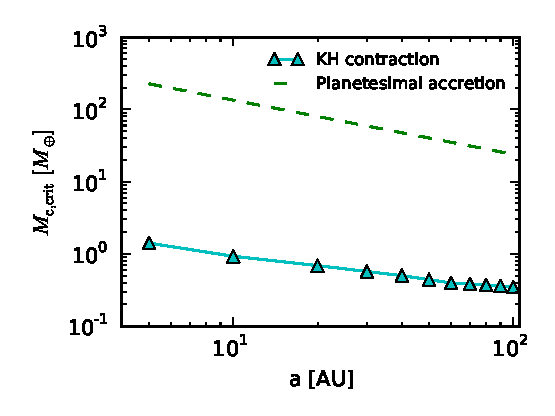
\includegraphics[width=0.5\textwidth]{../../figs/ModelAtmospheres/RadSelfGravRealEOS/Mc_vs_a_poly_raf2_paper.pdf}
%\vspace{-0.5in}
\caption{Comparison between the critical core mass $M_{\rm{crit, acc}}$ due to planetesimal accretion and the assumed fixed core mass when gas contraction dominates, for a growth time of $\tau=2.6$ Myrs. Our results yield lower core masses than in the standard case.}
\label{fig:raf2}
\end{figure}

We see that the critical core mass due to planetesimal accretion is smaller than in the case in which planetesimal accretion dominates the evolution of the atmosphere. This brings us to two conclusions. First, we confirm that planetesimal accretion can be safely ignored in our regime of interest. Secondly, this comparison tells us that it is easier and more efficient to form a planet by growing the core first, then accreting a massive envelope, rather than by growing the core and atmosphere in parallel. Moreover, our result represents a true, absolute minimum on the core mass that is needed to form a giant planet during the lifetime of the protoplanetary disk, as our core no longer grows.

% \textbf{This works for this particular choice of core, disk etc. conditions, and I am expecting it to work for most of our parameter space, but it would probably be good to explore this numerically, at least to order of magnitude, with the estimates we have.} 

%This means that for large core masses, planetesimal accretion will lead to runaway gas accretion before gas contraction starts dominating, and hence our model is not applicable in that regime. However, we have found in section \ref{critcore} that unstable atmospheres collapse occurs within the life time of the disk for protoplanetary cores smaller than this. 

As a final check, we investigate whether planetesimal accretion during the gas contraction phase at the rate $\dot{M}_{\rm{KH}}$ imposed by the condition that $L_{\rm{acc}}<L_{\rm{KH}}$ can alter the core mass enough to affect the time evolution of the atmosphere. We can quantitatively estimate the increase in core mass as 

\begin{equation}
\label{eq:cminc}
\Delta M_{\rm{c}} = \int_0^{t_{\rm{crit}}} \dot{M_{\rm{c}}} dt \approx \sum_i \dot{M_{\rm{c}}}_i \Delta t_i,
\end{equation}
 
 \noindent where $t_{\rm{crit}}$ is the time elapsed until runaway gas accretion commences, and the accretion rate $ \dot{M_{\rm{c}}}_i $ is given by 
 
 \begin{equation}
 \label{eq:Mdotexp}
 \dot{M_{\rm{c}}}_i =\frac{L_i R\co}{G M_{\rm{c}}} 
 \end{equation}
 
 \noindent from equation (\ref{eq:Lacc}), with $L_i$ the luminosity of the atmosphere at time $t_i$ in our model. For $M_{\rm{c}}=10 M_{\oplus}$, we find $\Delta M_{\rm{c}} \approx 0.2 M_{\oplus}$. This mass increase is therefore negligible in comparison with the initial core mass. It follows that a significant increase in core mass that could potentially alter the time evolution of the atmosphere would occur on a longer time scale than the mass-doubling time for the unperturbed atmosphere. Therefore, the time evolution of the atmosphere is insensitive to core mass changes at a rate imposed by the assumption that $L_{\rm{acc}}<L_{\rm{KH}}$.

%\section{Model Validity??? \textbf{(for now, in lack of a better title)}}
%
%\textbf{Discuss geometric effects (spherical symmetry in the inner disk), opacity effects (also in the 	inner disk) and planetesimal accretion; from this build the parameter space where the model is 	valid and confirm from the plots in the previous section that this is where we're looking. Part of the text regarding the planetesimal accretion discussion is below, as initially written for Paper I}
%
%\subsection{Geometric Effects}
%\subsection{Opacity Effects}
%
%
%\section{Discussion}
%\label{discussion}

%In this section we discuss the parameter space of validity of our model. We calculate the conditions under which planetesimal accretion can be ignored, and review the effects of some of the approximations that come into our model.
%
%  
 \section{Conclusions}
 \label{conclusions}
 
 In this paper we have studied giant planet formation under the assumption that the planetesimal accretion rate is negligible and the atmosphere evolution is dominated by gas contraction. We have used the model developed in Piso \& Youdin (in prep.) to build atmosphere profiles assuming that the nebular gas obeys a realistic equation of state that takes into account non-ideal effects. We found that the variations in the adiabatic index due to the realistic equation of state result in a significantly larger crossover time, and therefore critical core mass, when compared to an ideal gas polytrope. While for an ideal diatomic gas the minimum core mass to form a giant planet under the assumptions of our model is lower than the typically quoted value of $10 M_{\oplus}$ (see Piso \& Youdin in prep.), the inclusion of non-ideal effects brings this values back to around $10 M_{\oplus}$,
 
 We also compared our results to standard studies that assume that the evolution of the gaseous envelope is dominated by planetesimal accretion. We found that that our model yields lower core masses than the standard results. It is therefore easier to form a giant planet by growing the core first, then reducing the planetesimal accretion rate and let the atmosphere evolve on a Kelvin-Helmholtz time scale. Moreover, our results represent a true minimum on the core mass needed to form a giant planet during the typical lifetime of a protoplanetary disk.
 
% In this paper we have studied the formation of giant planet atmospheres under the assumption that Kelvin-Helmoholtz gas contraction dominates the luminosity evolution of the atmosphere over planetesimal accretion. We built quasi-static two-layer atmosphere models with an inner convective region and an outer radiative region that matches smoothly onto the protoplanetary disk. We derived a cooling model to connect series of quasti-static atmospheres, and thus obtained an evolutionary history of the envelope. We defined the time at which unstable atmosphere collapse commences as $M_{\rm atm}(t)\sim M_{\rm c}$. From this we defined as ``critical core mass'' the minimum core mass for a protoplanet to initiate runaway gas accretion during the lifetime of the protoplanetary disk. We studied this minimum mass for a variety of disk conditions, nebular gas compositions and opacities. We found that the critical core mass decreases as we move further out in the disk, and is smaller for lower disk temperatures and opacities and for higher mean molecular weight of the gas. 
% 
% We find that the critical core mass to form a giant planet within the life time of the disk is smaller than the results yielded by studies that assume that the atmosphere evolution is dominated by the luminosity due to planetesimal accretion. We have showed that the planetesimal accretion rate needed to grow the core on a typical disk time scale is larger than the expected planetesimal accretion rates at large separations. As such, it is faster to form a planet by growing the core first in a fast planetesimal accretion regime (e.g., the core forms in the inner disk, then migrates outwards), then significantly reduce planetesimal accretion and allow a massive atmosphere to accumulate. 
 
%Our study assumes that the protoplanetary core forms first, then it r
 
%---------------------------------------------------------------------------
\bibliographystyle{apj}
\bibliography{refs}

\appendix
\section{Equation of State Tables}\label{EOStables}

In this section we explain the procedure for extending and interpolating the \cite{saumon95} equation of state tables. The equation of state takes into account non ideal interactions, and includes physical treatments of dissociation and ionization. However, the \cite{saumon95} EOS tables only cover a relatively high range of temperatures and pressures: $2.10 < \log_{10} T(\rm{K})<7.06$ and $4<\log_{10}P$(dyn cm$^{-2})<19$. We consider cold disks, where the temperature and pressure drop to $\sim 20$ K and $\sim 10^{-4}$ dyn cm$^{-2}$, respectively (see equations (\ref{eq:diskb}) and (\ref{eq:Pd})). As such, it is necessary to extend the \cite{saumon95} EOS tables to lower temperature and pressure values.

We choose $\log_{10} T (\rm{K})=1$ and $ \log_{10}P$(dyn cm$^{-2})=-4.4$ as our lower boundaries for temperature and pressure, respectively. Our temperature and pressure grid becomes: $1 < \log_{10} T(\rm{K})<7.06$ and $-4.4<\log_{10}P$(dyn cm$^{-2})<19$. The other thermodynamic variables in the tables are calculated as follows.

\subsection{Hydrogen}

\label{hydrogen}

For a system of particles, the partition function can be written as the product of all partition functions associated with each type of energy that the system can have:

\begin{equation}
\label{eq:z}
Z=Z_t Z_r Z_v Z_e Z_n,
\end{equation}

\noindent where $Z_t$, $Z_r$, $Z_v$, $Z_e$ and $Z_n$ are the partition functions associated with translation, rotation, vibration, electronic excitation and nuclear excitation, respectively. For hydrogen, electronic and nuclear excitation are only significant at temperatures higher than our region of interest ($\theta_e \approx 12000$ K and $\theta_n >> \theta_e$, where $\theta_e$ and $\theta_n$ are the characteristic temperatures for electronic and nuclear excitation, respectively). As such, we will only take into account the translation, rotation and vibration of the hydrogen molecule:

\begin{equation}
\label{eq:zagain}
Z=Z_t Z_r Z_v
\end{equation} 

The partition function associated with the motion of the center of mass of the molecule is given by (in the classical limit):

\begin{equation}
\label{eq:Zt}
Z_t=(m/2 \beta \pi \hbar^2)^{3/2} V,
\end{equation}

\noindent where $\beta=1/(k T)$ and $V$ is the volume. The rotational partition function is generally written as:

\begin{equation}
\label{eq:Zr}
Z_r=\sum_0^\infty (2 j+1) \exp{\Big[\frac{-j (j+1)\Theta_r}{T}\Big]},
\end{equation}

\noindent where $\Theta_r$ is the characteristic temperature for rotational motion. In the case of hydrogen, $\Theta_r \approx 85$ K. However, molecular hydrogen occurs in two isomeric forms: orthohydrogen, with the proton spins aligned parallel to each other, and parahydrogen, with the proton spins aligned antiparallel. Parahydrogen can only a have symmetric (even) wave function associated with rotation, while orthohydrogen can only have an antisymmetric (odd) wave function associated with rotation (see section \ref{deladtable} for an explanation why). The rotational partition functions for ortho- and parahydrogen can thus be written as:

\begin{equation}
\label{eq:Zpara}
Z_{\rm{r,para}}=\frac{1}{2}\sum_0^\infty (1+(-1)^j) (2 j +1) \exp\Big[-\frac{j(j+1)\Theta_r}{T}\Big]
\end{equation}
and
\begin{equation}
\label{eq:Zortho}
Z_{\rm{r,ortho}}=\frac{3}{2}\sum_0^\infty (1-(-1)^j) (2 j +1) \exp\Big[-\frac{j(j+1)\Theta_r}{T}\Big]
\end{equation}

The factor of 3 above accounts for the three-fold degeneracy of the ortho state.

 When the two isomers are in equilibrium, the combined partition function is given by the sum of the individual partition functions, $Z_{\rm r}=Z_{\rm{r, ortho}}+Z_{\rm{r,para}}$ and can be written as:

\begin{equation}
\label{eq:Zrspin}
Z_r=\sum_0^\infty (2-(-1)^j) (2j+1) \exp{\Big[\frac{-j (j+1) \Theta_r}{T}\Big]}
\end{equation}

In our range of temperatures of interest, we found that $Z_r$ converges after about 25 terms in the series.


Finally, the partition function for vibrational motion is given by:

\begin{equation}
\label{eq:Zv}
Z_v=[1-\exp{(\theta_v/T)}]^{-1},
\end{equation}

\noindent where $\theta_v$ is the characteristic temperature for vibrational motion, $\theta_v \approx 6140$ K for hydrogen. 

If the partition function of a system of $N$ particles is known in terms of $(V, T, N)$, the internal energy and entropy of the system can be determined as follows:

\begin{equation}
\label{eq:U}
U_N=k T^2 \Big(\frac{\partial \log{Z}}{\partial T}\Big)_{V, N}
\end{equation}

\begin{equation}
\label{eq:S}
S_N=k \log{Z} + \frac{U_N}{T}
\end{equation}

The energy, and entropy per mass and specific heat capacity will subsequently be:

\begin{equation}
\label{eq:u}
U=\mathcal{R} T^2 \Big(\frac{\partial \log{Z}}{\partial T}\Big)_{V, N}
\end{equation}

\begin{equation}
\label{eq:s}
S=\mathcal{R} \log{Z} + \frac{U}{T}
\end{equation}

\begin{equation}
\label{eq:cv}
C_v=\Big(\frac{\partial U}{\partial T}\Big)_{V, N}
\end{equation}


Since $Z=Z_t Z_r Z_v$, it is easy to notice that $U=U_t+U_r+U_v$ and $S=S_t+S_r+S_v$, where $U_t$, $U_r$, $U_v$, $S_t$, $S_r$, $S_v$ are the quantities corresponding to the individual translation, rotation and partition functions, respectively.

It can be shown that the entropy per mass due to translational motion can be expressed as:

\begin{equation}
\label{eq:st}
S_t=\mathcal{R} \Big[ \frac{5}{2} \ln{T} - \ln{P} + \ln \Big( \frac{(2 \pi)^{3/2} \mathcal{R}^{5/2} \mu^4}{h^3}\Big) +\frac{5}{2} \Big]
\end{equation}

\noindent with $\mu$ the mean molecular weight. Equation (\ref{eq:st}) is known as the Sackur-Tetrode formula, and it is only applicable to an ideal gas. It can also be easily shown that the internal energy per mass due to translational motion is given by:

\begin{equation}
\label{eq:ut}
U_t=\frac{3}{2} \mathcal{R} T
\end{equation}

Putting all of the above together, we can now evaluate the thermodynamic quantities needed to extend the \cite{saumon95} EOS tables to low temperatures and pressures.

\begin{enumerate}

\item{\textbf{Density.}} In the low temperature, low pressure regime, hydrogen is molecular and behaves like an ideal gas. As such, the density in this region follows the ideal gas law $P=\rho \mathcal{R} T$.
\item{\textbf{Internal energy per mass.}} $U=U_t+U_r+U_v$, where $U_t$ is given by equation (\ref{eq:ut}), and $U_r$, $U_v$ are determined using equations (\ref{eq:u}), (\ref{eq:Zrspin}) and (\ref{eq:Zv}) above.
\item{\textbf{Entropy per unit mass}}. Similarly, $S=S_t+S_r+S_v$, where $S_t$ is given by equation (\ref{eq:st}), and $S_r$, $S_v$ can be determined from equation (\ref{eq:s}) and the calculated expressions for $U_r$ and $U_v$, respectively.
\item{\textbf{Entropy logarithmic derivatives}}. The logarithmic derivatives $S_T$ and $S_P$ are given by:

\begin{equation}
\label{eq:sT}
S_T=\frac{\partial \log{S}}{\partial \log{T}} \Big |_P
\end{equation}

\noindent and

\begin{equation}
\label{eq:sP}
S_T=\frac{\partial \log{S}}{\partial \log{P}} \Big |_T
\end{equation}

We calculate $S_T$ and $S_P$ using the table values for $S$, $T$ and $P$, and a linear central difference formula. 

\item{\textbf{Adiabatic gradient $\nabla_{ad}$}}. The adiabatic gradient is defined as:

\begin{equation}
\label{eq:deladSP}
\nabla_{ad}=\frac{\partial \log{T}}{\partial \log{P}} \Big |_S = -\frac{S_P}{S_T}
\end{equation}

We evaluate it from the tabulated values for $S_T$ and $S_P$ determined above. Figure 1 shows a contour plot of the adiabatic index for the extended EOS table, while the black lines represent constant entropy curves. The upper right part of the plot ($\log T>2.1$ and $\log P>4$) is based on the \cite{saumon95} EOS table, while the rest of the plot is our extension. We see that the two tables join smoothly for entropy curves between $8.80<\log{S}$(K g$^{-1})<9.07$.

\end{enumerate}

\begin{figure}[h!]
\centering
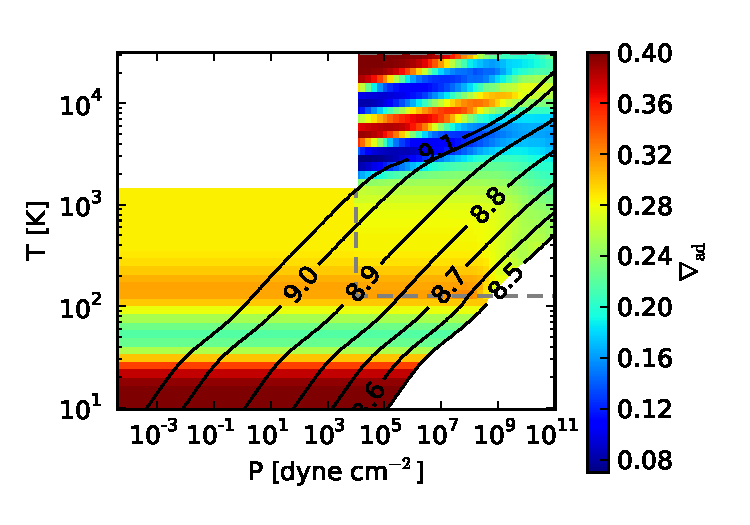
\includegraphics[scale=.8]{../../figs/EOS/delad_S_H.pdf}
\caption{Contour plot of the adiabatic gradient $\delad$ for the hydrogen extended table. The black curves represent constant entropy curves.}
\end{figure}

\subsection{Helium}

We extend the helium EOS tables based on a similar procedure. Since helium is primarily neutral and atomic at low temperatures and pressures, we treat it as an ideal monoatomic gas, and subsequently only take into account the translational components of the necessary thermodynamic quantities (see subsection \ref{hydrogen} above for details). The analogous $\nabla_{ad}$ contour plot for helium can be seen in Figure 2. We notice that, in the case of helium, the original and extended table join smoothly for entropy curves between $8.29<\log{S}$(K g$^{-1})<8.77$.

\begin{figure}[h!]
\centering
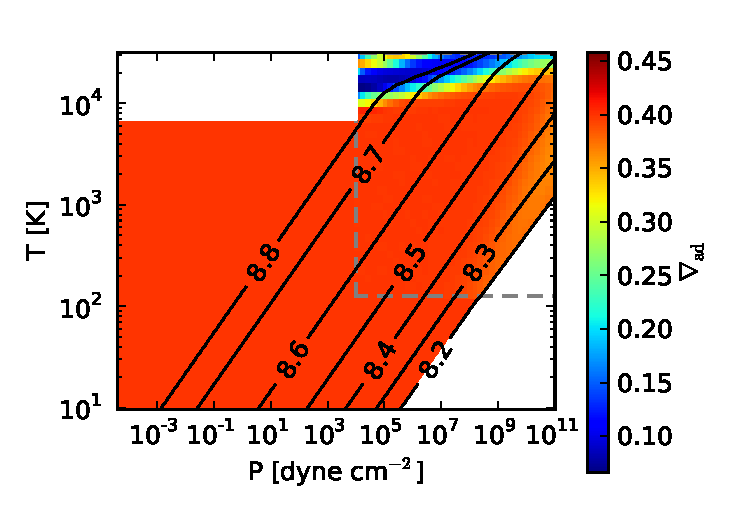
\includegraphics[scale=.8]{../../figs/EOS/delad_S_He.pdf}
\caption{Contour plot for the adiabatic gradient $\delad$ for the helium extended table. The black curves represent constant entropy curves.}
\end{figure}

\vspace{0.2in}

Lastly, we obtain the equation of state tables for the hydrogen-helium mixture thorough the procedure described in \citet{saumon95}, for a helium mass fraction $Y=0.3$.

%Using equation (\ref{eq:upartition}) we therefore recover the standard result $U_{\rm r}=\mathcal{R} T$ (refs). Furthermore, we know that the internal energy and entropy per unit mass associated with translation are given by $U_{\rm t}=\frac{3}{2} \mathcal{R}$ and $C_{\rm{v,t}}=\frac{3}{2}\mathcal{R}$, respectively, and so we are able to calculate the total internal energy and specific heat of a diatomic molecule as a function of temperature. An example of the variation of heat capacity with temperature is shown in \citet{kittel}, chapter 3. 

%The partition function associated with rotation is generally written as:
%
%\begin{equation}
%\label{eq:Zr}
%Z_{\rm r}=\sum_0^\infty (2 j +1) \exp\Big[-\frac{j(j+1)\Theta_r}{T}\Big],
%\end{equation}
%with $j$ the angular momentum quantum number \citep{kittel}. Various thermodynamic quantities can be derived from the partition function. For example, the internal energy per unit mass can be written as:
%
%\begin{equation}
%\label{eq:upartition}
%u_{\rm r}=\mathcal{R}T^2 \frac{\partial \log Z}{\partial T}
%\end{equation}
%
%The specific heat at constant volume then easily follows as
%
%\begin{equation}
%\label{eq:cvpartition}
%c_{\rm{v,r}}=\Big(\frac{\partial u}{\partial T}\Big)_V
%\end{equation} 


 







\section{Adiabatic Gradient during Partial Ionization}\label{deladioniz}

For a partially ionized gas, the total internal energy includes contributions from the individual internal energies of neutral atoms, ions and electrons, as well as from the ionization energy. Specifically, if we denote the internal energies of neutral hydrogen, protons and electrons as $U_{H}$, $U_+$ and $U_e$, respectively, then the total internal energy of the gas is given by:

\begin{equation}
U=U_H+U_+ + U_e + x \chi,
\end{equation}

\noindent where $x$ is the ionization fraction and $\chi$ is the ionization energy (equal to -13.6 eV for hydrogen). The ionization fraction can be determined from the Saha equation (see e.g., \citealt{kippenhahn90}).

\begin{equation}
\label{eq:saha}
\frac{x^2}{1-x} \frac{\rho}{m_H}=\frac{(2 \pi m_e k_B T)^{3/2}}{h^3} e^{-\chi/k_B T},
\end{equation}

\noindent where $m_e$ is the mass of the electron and $h$ is Planck's constant. It can be seen from the Saha equation that the ionization fraction depends only on the gas temperature and density: $x=x(T, \rho)$. As such, all the thermodynamic quantities also depend only on the gas temperature and density, and hence on the equation of state. The adiabatic gradient is given by (see \citealt{kippenhahn90}, chapter 14 for a derivation):

\begin{equation}
\delad=\frac{2+x (1-x) \Phi_H}{5+x (1-x) \Phi_H^2},
\end{equation} 
with $\Phi_H=\frac{5}{2}+\frac{\chi}{k T}$. Figure \ref{fig:deladion} shows the behavior of $\delad$ for partially ionized hydrogen. We recover $\delad=2/5$ for $x=0$ (pure atomic hydrogen) and $x=1$ (fully ionized plasma). The adiabatic gradient decreases significantly for intermediate values of $x$, becoming smaller than 0.1 at its minimum (for $x=0.5$). 

\begin{figure}[h]
\centering
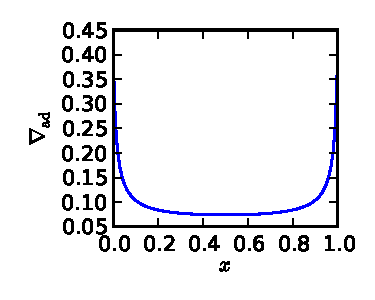
\includegraphics[width=0.5\textwidth]{../../figs/ModelAtmospheres/RadSelfGravRealEOS/EOSeffects/delad_ionization.pdf}
%%\vspace{-0.5in}
\caption{Adiabatic gradient as a function of the hydrogen ionization fraction $x$. The adiabatic gradient is $\delad=2/5$ for pure atomic hydrogen ($x=0$) and fully ionized hydrogen ($x=1$), and drops to low values during partial ionization.}
\label{fig:deladion}
\end{figure}



\end{document}




